% Options for packages loaded elsewhere
\PassOptionsToPackage{unicode}{hyperref}
\PassOptionsToPackage{hyphens}{url}
%
\documentclass[
  11pt,
  man,floatsintext]{apa6}
\usepackage{amsmath,amssymb}
\usepackage{iftex}
\ifPDFTeX
  \usepackage[T1]{fontenc}
  \usepackage[utf8]{inputenc}
  \usepackage{textcomp} % provide euro and other symbols
\else % if luatex or xetex
  \usepackage{unicode-math} % this also loads fontspec
  \defaultfontfeatures{Scale=MatchLowercase}
  \defaultfontfeatures[\rmfamily]{Ligatures=TeX,Scale=1}
\fi
\usepackage{lmodern}
\ifPDFTeX\else
  % xetex/luatex font selection
\fi
% Use upquote if available, for straight quotes in verbatim environments
\IfFileExists{upquote.sty}{\usepackage{upquote}}{}
\IfFileExists{microtype.sty}{% use microtype if available
  \usepackage[]{microtype}
  \UseMicrotypeSet[protrusion]{basicmath} % disable protrusion for tt fonts
}{}
\makeatletter
\@ifundefined{KOMAClassName}{% if non-KOMA class
  \IfFileExists{parskip.sty}{%
    \usepackage{parskip}
  }{% else
    \setlength{\parindent}{0pt}
    \setlength{\parskip}{6pt plus 2pt minus 1pt}}
}{% if KOMA class
  \KOMAoptions{parskip=half}}
\makeatother
\usepackage{xcolor}
\usepackage{graphicx}
\makeatletter
\def\maxwidth{\ifdim\Gin@nat@width>\linewidth\linewidth\else\Gin@nat@width\fi}
\def\maxheight{\ifdim\Gin@nat@height>\textheight\textheight\else\Gin@nat@height\fi}
\makeatother
% Scale images if necessary, so that they will not overflow the page
% margins by default, and it is still possible to overwrite the defaults
% using explicit options in \includegraphics[width, height, ...]{}
\setkeys{Gin}{width=\maxwidth,height=\maxheight,keepaspectratio}
% Set default figure placement to htbp
\makeatletter
\def\fps@figure{htbp}
\makeatother
\setlength{\emergencystretch}{3em} % prevent overfull lines
\providecommand{\tightlist}{%
  \setlength{\itemsep}{0pt}\setlength{\parskip}{0pt}}
\setcounter{secnumdepth}{-\maxdimen} % remove section numbering
% Make \paragraph and \subparagraph free-standing
\ifx\paragraph\undefined\else
  \let\oldparagraph\paragraph
  \renewcommand{\paragraph}[1]{\oldparagraph{#1}\mbox{}}
\fi
\ifx\subparagraph\undefined\else
  \let\oldsubparagraph\subparagraph
  \renewcommand{\subparagraph}[1]{\oldsubparagraph{#1}\mbox{}}
\fi
\ifLuaTeX
\usepackage[bidi=basic]{babel}
\else
\usepackage[bidi=default]{babel}
\fi
\babelprovide[main,import]{english}
% get rid of language-specific shorthands (see #6817):
\let\LanguageShortHands\languageshorthands
\def\languageshorthands#1{}
\usepackage{fontspec}

%% Pandoc can only set 10, 11, 12 pt
%% uncomment below to set fontsize
%\usepackage[fontsize=13pt]{scrextend}

%\setmainfont{Calibri} % Set main font for latin characters

\setlength{\parskip}{0.15cm} % Set space between paragraphs
%\linespread{1.2}\selectfont % Set line height
%\usepackage[doublespacing]{setspace} % Use double space without changing footnotes line height

%% Special font for IPA
%% Make sure "Doulos SIL" is installed on your computer
%% For other typefaces supporting IPA symbols, see
%% https://en.wikipedia.org/wiki/International_Phonetic_Alphabet#Typefaces
\newfontfamily\ipa{Doulos SIL} % Font for IPA symbols
\DeclareTextFontCommand{\ipatext}{\ipa}



%%%         Section for CJK Characters                   %%%
%%%   You may want to uncomment the code below if        %%%
%%%   you're writing this document with CJK characters   %%%

%\usepackage{xeCJK}  % Uncomment for using CJK characters
%% Set main font for CJK characters
%% Make sure your system has the font set
%\setCJKmainfont[
%	BoldFont={HanWangHeiHeavy}  % Set font for CJK boldface
%    ]{標楷體}    % Set font for normal CJK
%% Some Traditional Chinese fonts: AR PL KaitiM Big5, PingFang TC, Noto Sans CJK TC
%\XeTeXlinebreaklocale "zh"
%\XeTeXlinebreakskip = 0pt plus 1pt

%% Added by Florian to make biblatex and its \refsection work since pandoc does not parse 
%% content within latex environments. \refsection in turn is required to allow authors
%% to have multiple separate bibliographies (here: one for main text and one for SI).
%%
%% For some reasons it does seem to be necessary to reload the bibpackage here since
%% ---at least for my system---adding the following to the YAML header instead does
%% not seem to work:
%%
%%    biblio-style: apa
%%    biblatexoptions: [backend=biber,maxbibnames=999,style=apa]
%% 
%% curiously removing the following from the YAML header:
%%
%%     citation_package: biblatex
%%
%% makes knitr (or pandoc?) revert back to the default bibtex treatment, which does 
%% not allow multiple bibliographies.
\usepackage[backend=biber,maxbibnames=999,style=apa]{biblatex}
\addbibresource{latex-stuff/library.bib}
\newcommand{\brefsection}{\begin{refsection}}
\newcommand{\erefsection}{\end{refsection}}
% Manuscript styling
\usepackage{upgreek}
\captionsetup{font=singlespacing,justification=justified}

% Table formatting
\usepackage{longtable}
\usepackage{lscape}
% \usepackage[counterclockwise]{rotating}   % Landscape page setup for large tables
\usepackage{multirow}		% Table styling
\usepackage{tabularx}		% Control Column width
\usepackage[flushleft]{threeparttable}	% Allows for three part tables with a specified notes section
\usepackage{threeparttablex}            % Lets threeparttable work with longtable

% Create new environments so endfloat can handle them
% \newenvironment{ltable}
%   {\begin{landscape}\centering\begin{threeparttable}}
%   {\end{threeparttable}\end{landscape}}
\newenvironment{lltable}{\begin{landscape}\centering\begin{ThreePartTable}}{\end{ThreePartTable}\end{landscape}}

% Enables adjusting longtable caption width to table width
% Solution found at http://golatex.de/longtable-mit-caption-so-breit-wie-die-tabelle-t15767.html
\makeatletter
\newcommand\LastLTentrywidth{1em}
\newlength\longtablewidth
\setlength{\longtablewidth}{1in}
\newcommand{\getlongtablewidth}{\begingroup \ifcsname LT@\roman{LT@tables}\endcsname \global\longtablewidth=0pt \renewcommand{\LT@entry}[2]{\global\advance\longtablewidth by ##2\relax\gdef\LastLTentrywidth{##2}}\@nameuse{LT@\roman{LT@tables}} \fi \endgroup}

% \setlength{\parindent}{0.5in}
% \setlength{\parskip}{0pt plus 0pt minus 0pt}

% Overwrite redefinition of paragraph and subparagraph by the default LaTeX template
% See https://github.com/crsh/papaja/issues/292
\makeatletter
\renewcommand{\paragraph}{\@startsection{paragraph}{4}{\parindent}%
  {0\baselineskip \@plus 0.2ex \@minus 0.2ex}%
  {-1em}%
  {\normalfont\normalsize\bfseries\itshape\typesectitle}}

\renewcommand{\subparagraph}[1]{\@startsection{subparagraph}{5}{1em}%
  {0\baselineskip \@plus 0.2ex \@minus 0.2ex}%
  {-\z@\relax}%
  {\normalfont\normalsize\itshape\hspace{\parindent}{#1}\textit{\addperi}}{\relax}}
\makeatother

% \usepackage{etoolbox}
\makeatletter
\patchcmd{\HyOrg@maketitle}
  {\section{\normalfont\normalsize\abstractname}}
  {\section*{\normalfont\normalsize\abstractname}}
  {}{\typeout{Failed to patch abstract.}}
\patchcmd{\HyOrg@maketitle}
  {\section{\protect\normalfont{\@title}}}
  {\section*{\protect\normalfont{\@title}}}
  {}{\typeout{Failed to patch title.}}
\makeatother

\usepackage{xpatch}
\makeatletter
\xapptocmd\appendix
  {\xapptocmd\section
    {\addcontentsline{toc}{section}{\appendixname\ifoneappendix\else~\theappendix\fi\\: #1}}
    {}{\InnerPatchFailed}%
  }
{}{\PatchFailed}
\keywords{speech perception; computational model; accent adaptation; perceptual recalibration}
\usepackage{csquotes}
\usepackage{animate}
\usepackage{amsmath}
\usepackage{tikz}
\usetikzlibrary{bayesnet}
\usepackage{booktabs}
\usepackage{siunitx}
\usepackage{soul}
\usepackage{tabto}
\usepackage{xcolor}
\usepackage{placeins}
\setstcolor{red}
\usepackage{sectsty}
\sectionfont{\color{black}}
\subsectionfont{\color{black}}
\subsubsectionfont{\color{black}}
\usepackage{setspace}\doublespacing
\usepackage[labelformat=simple]{subcaption}
\usepackage{hyperref}
\ifLuaTeX
  \usepackage{selnolig}  % disable illegal ligatures
\fi
\usepackage[]{biblatex}
\addbibresource{latex-stuff/library.bib}
\addbibresource{latex-stuff/r-references.bib}
\IfFileExists{bookmark.sty}{\usepackage{bookmark}}{\usepackage{hyperref}}
\IfFileExists{xurl.sty}{\usepackage{xurl}}{} % add URL line breaks if available
\urlstyle{same}
\hypersetup{
  pdftitle={What we do (not) know about the mechanisms underlying adaptive speech perception: A computational framework and review},
  pdfauthor={Xin Xie1,2, T. Florian Jaeger2,3, \& Chigusa Kurumada2},
  pdflang={en-EN},
  pdfkeywords={speech perception; computational model; accent adaptation; perceptual recalibration},
  hidelinks,
  pdfcreator={LaTeX via pandoc}}

\title{What we do (not) know about the mechanisms underlying adaptive speech perception: A computational framework and review}
\author{Xin Xie\textsuperscript{1,2}, T. Florian Jaeger\textsuperscript{2,3}, \& Chigusa Kurumada\textsuperscript{2}}
\date{July 21, 2023}


\shorttitle{Exposure effects in speech perception}

\authornote{

We are grateful to Meghan Clayards and Eleanor Chodroff for sharing their data in an accessible format, and for helping prepare their data for this study. We thank the participants in the 2021 summer `mega-lab' meetings for many insightful discussions that shaped the perspectives discussed here (all mistakes remain our own). This includes, in particular, Ann Bradlow, Melissa Baese-Berk, Eleanor Chodroff, Jennifer Cole, Laura Dilley, James McQueen, Arty Samuel, and Rachel Theodore. We also owe special thanks, and insights, to feedback from Marc Allassonnière-Tang, Zach Burchill, Wednesday Bushong, Shawn Cummings, Seth Cutler, Volya Kapatsinski, Jing Liu, Gerda Melnik, Anna Persson, Paula Rubio Fernandez, and Rachel Sabatello. Finally, we thank the reviewers and editors who provided particularly constructive critiques, gave us room to develop our ideas, and showed patience throughout the process of preparing and improving this manuscript.

Correspondence concerning this article should be addressed to Xin Xie, 3151 Social Science Plaza B, University of California, Irvine CA 92697--5100. E-mail: \href{mailto:xxie14@uci.edu}{\nolinkurl{xxie14@uci.edu}}

}

\affiliation{\vspace{0.5cm}\textsuperscript{1} Language Science, University of California, Irvine\\\textsuperscript{2} Brain and Cognitive Sciences, University of Rochester\\\textsuperscript{3} Computer Science, University of Rochester}

\abstract{%
Speech from unfamiliar talkers can be difficult to comprehend initially. These difficulties tend to dissipate with exposure, sometimes within minutes or less. Adaptivity in response to unfamiliar input is now considered a fundamental property of speech perception, and research over the past two decades has made substantial progress in identifying its characteristics. The \emph{mechanisms} underlying adaptive speech perception, however, remain unknown. Past work has attributed facilitatory effects of exposure to any one of three qualitatively different hypothesized mechanisms: (1) low-level, pre-linguistic, signal normalization, (2) changes in/selection of linguistic representations, or (3) changes in post-perceptual decision-making. Direct comparisons of these hypotheses, or combinations thereof, have been lacking. We describe a general computational framework for adaptive speech perception (ASP) that---for the first time---implements all three mechanisms. We demonstrate how the framework can be used to derive predictions for experiments on perception from the acoustic properties of the stimuli. Using this approach, we find that---at the level of data analysis presently employed by most studies in the field---the signature results of influential experimental paradigms do not distinguish between the three mechanisms. This highlights the need for a change in research practices, so that future experiments provide more informative results. We recommend specific changes to experimental paradigms and data analysis. All data and code for this study are shared via OSF, including the R markdown document that this article is generated from, and an R library that implements the models we present.
}



\begin{document}
\maketitle

\setcounter{secnumdepth}{5}
\renewcommand{\thesubfigure}{\textbf{\Alph{subfigure})}}

\brefsection

\setcounter{page}{1}

\hypertarget{introduction}{%
\section{Introduction}\label{introduction}}

How human listeners are able to infer meaning from speech is a central question in cognitive and neurosciences. The computational complexity of spoken language understanding becomes most apparent when a talker's pronunciations---and thus the mapping of acoustic input to linguistic categories and meaning---strongly deviate from listeners' expectations. This might occur, for example, when listening to a talker with an unfamiliar regional or non-native accent, or a patient with apraxia or dysarthria. The same fundamental challenge is, however, present even during seemingly effortless comprehension. Even among talkers who share similar language backgrounds, the mapping between the acoustic input and linguistic categories can vary substantially between talkers due to both physiology (e.g., vocal tract size and shape) and socio-cultural factors (e.g., social identity and language background). As a consequence, one talker's pronunciation of, say, the sound category /s/ (as in \emph{sip}) can be acoustically more similar to another talker's production of \(/\ipatext{ʃ}/\) \autocite[as in \emph{ship},][]{newman2001}. How we manage to understand each other despite such cross-talker differences has remained one of the perennial puzzles in research on speech perception \autocite[where it is known as part of the infamous \emph{lack of invariance} problem,][]{liberman1967}.

This article presents a general computational framework---which we refer to as \emph{ASP} for \emph{adaptive speech perception}---that helps address this question. ASP grew out of our long-term goal to contribute to the development of stronger theories, affording decisive comparisons between alternative hypotheses about the mechanisms underlying speech perception \autocite[in the tradition of ``strong inference'' approaches to scientific inquiry,][]{platt1964}. We identify the three most influential hypotheses about the mechanisms that allow listeners to overcome cross-talker variability (Figure \ref{fig:overview}). These three hypotheses---described below---entail fundamentally different cognitive abilities and neural architectures, with far-reaching consequences for theories of speech perception, linguistics, and the malleability of neural representations more generally. ASP is the first to formalize and implement all three of these mechanisms in a common computational framework. This responds to a need identified in recent reviews to better characterize the mechanisms of adaptive speech perception \autocite{baeseberk2020,kurumada-roettger2021,johnson-sjerps2021,quam-creel2021,stilp2020,weatherholtz-jaeger2016}.

\begin{figure}[h]
\begin{center}
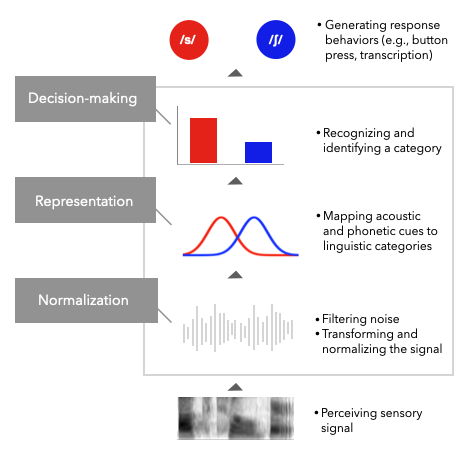
\includegraphics[width=0.6\columnwidth]{../figures/diagrams/overview-of-three-mechanisms.png}
\caption{Listeners' recognition of speech categories are typically assumed to involve at least three types of mechanisms: 1) the acoustic input is transformed by low-level normalization processes into the perceptual cues that form the input to categorization, 2) category representations describe the mapping between these perceptual and linguistic categories (here $C_1$ and $C_2$), and 3) decision-making mechanisms allow additional, stimulus-independent, biases to affect recognition. Any of these three mechanisms can in theory be affected by recent experience. It is unknown which (combination) of the three mechanisms underlie these changes and how the engagement of different mechanisms depends on, for instance, stimulus properties, task demands, and individual differences between listeners.}\label{fig:overview}
\end{center}
\end{figure}

While the three hypotheses in Figure \ref{fig:overview} have largely been pursued in separate lines of research, they are not mutually exclusive. This raises questions as to whether adaptive speech perception is the result of \emph{combinations} of these mechanisms, and (if so) how the relative engagement of these mechanisms depends on, for instance, stimulus properties, task demands, or individual differences between listeners. ASP can be used to address these questions. Researchers can, for example, use ASP to predict adaptive changes in speech perception while `switching off' individual change mechanisms---making it possible to test whether any of the three mechanisms is \emph{sufficient} to explain a given result---or to predict changes from weighted combinations of all three mechanisms. Future work could use ASP, for example, to investigate whether specific instances of impaired adaptation \autocites[as seen, e.g., in children with dyslexia,][]{gabay2021,ozernov-palchik2021} arise from auditory, linguistic, or cognitive sources---an important prerequisite for devising more effective interventions/treatments.

For the present article, we have three more immediate goals. The first part of this article introduces the ASP framework, along with visual demonstrations and animations. We take a deliberately tutorial-like approach so to help researchers apply ASP to their own experiments. All data and code for this article can be downloaded from the Open Science Framework at \url{https://osf.io/q7gjp/}. The article is written in R markdown, allowing readers to replicate our analyses with the press of a button using freely available software \autocites{R}[see supplementary information for detailed software requirements]{RStudio}. Readers can also revisit any of the assumptions we make---e.g., changing parameterizations of our models, or substituting alternative models \autocite[see also][]{tan2021}. We welcome questions about the code, including the accompanying \texttt{R} library.

Second, we demonstrate one way in which computational frameworks like ASP can advance theories of speech perception. We simulate human recognition for two influential experimental paradigms under each of the three hypothesized mechanisms. The first paradigm---\emph{perceptual recalibration} \autocites[e.g.,][]{kraljic-samuel2006,reinisch-holt2013,samuel2016,vroomen-baart2009}---tends to employ a small set of exposure and test stimuli that are phonetically manipulated to form a single perceptual continuum. This property makes such experiments comparatively easy to understand and model, and thus suitable as an initial case study. The second paradigm---\emph{adaptation to second language (L2) accents} \autocites[e.g.,][]{bradlow-bent2008,hernandez2019,tzeng2016,sidaras2009,xie2016jep,zheng-samuel2020}---introduces a greater degree of complexity for both the listener and the researcher. Stimuli for these experiments tend to exhibit the full range of naturally occurring phonetic variability, introducing listeners to novel phonetic cues, differences in cue weightings, and other complex changes in the mapping from acoustics to linguistic categories.

We find that, contrary to common assumptions, the signature findings of both paradigms are qualitatively compatible with \emph{any} of the three hypothesized change mechanisms. Beyond the immediate consequences for research on perceptual recalibration and accent adaptation, this demonstrates how ASP can inform and revise intuitions about the mechanisms underlying adaptive speech perception. The R code for our case studies further serves as a template for experimenters interested in understanding the theoretical implications of their results while reducing the need for ad-hoc reasoning.

Finally, we discuss how computationally-guided behavioral and neuroimaging research can advance future work. We show that the empirical indeterminacy of many existing findings is due to the level of analysis employed in most research on adaptive speech perception. We propose new standards of experimental design and data analysis that will more effectively distinguish between competing hypotheses about the relative engagement of different mechanisms. But first some background.

\hypertarget{the-state-of-the-fields}{%
\subsection{The state of the field(s)}\label{the-state-of-the-fields}}

Research over the past decades has identified adaptive changes in speech perception to be a key component in listeners' ability to overcome cross-talker differences. Although speech perception can initially be slower and/or less accurate when listeners encounter an unfamiliar talker with unexpected pronunciations, these processing difficulties tend to reduce with exposure \autocites[e.g.,][]{bradlow-bent2008,nygaard1994,Perrachione2016,sidaras2009,wade2007,weil2001a,xie2021jep}. Remarkably, substantial improvements---such as reduced processing times or increased accuracy of recognition---can occur within minutes or less \autocite{clarke-garrett2004,munro-derwing1995,xie2018jasa}. Even a context as brief as a single utterance can be sufficient to change perception and segmentation of ambiguous speech, blurring the distinction between processing and adaptation \autocites[e.g., categorizing a Dutch ambiguous /m?t/ embedded in an utterance with fast or slow speech as either ``mat'' or ``maat'',][]{bosker2017}[see also][]{kluender1988,newman-sawusch1996,sawusch-newman2000,sjerps2011}. Yet, adaptive changes after only a few words of exposure can sometimes last for days, if not longer \autocites{eisner-mcqueen2006,samuel2021,xie2018lcn}[see also][]{goldinger1996}.

In short, listeners' ability to adapt based on recent input is now considered a central part of human speech perception, and substantial progress has been made in identifying its empirical properties and constraints \autocites[for comprehensive reviews, see][]{baeseberk2020,johnson-sjerps2021,tzeng2021,quam-creel2021,stilp2020}. Despite these substantial advances, however, \textbf{it remains unclear \emph{how}---through what mechanisms---recent exposure comes to facilitate spoken language understanding.} This is not due to a lack of theoretical proposals. Across cognitive sciences and neurosciences, there are now dozens of competing perspectives. However, contrastive comparisons between proposals have largely been lacking. Two inter-related factors seem to contribute to this: (1) many proposals---including some of our own past work---remain under-specified, constituting informal hypotheses rather than theories or models that lend themselves to strong contrastive tests; (2) there is a tendency, particularly in behavioral research, to focus on characterizing properties of adaptive speech perception rather than on identifying the underlying cognitive and neural architectures \autocites[but see][]{apfelbaum-mcmurray2015,chodroff-wilson2020,harmon2019,hoffmanbion-escudero2007,kleinschmidt-jaeger2015,kiefte-nearey2019,lehet-holt2020,mcmurray-jongman2011,xie2021cognition}. As a consequence, different hypotheses are often \emph{assumed} rather than tested, with different lines of research making different (implicit) assumptions, sometimes co-existing for decades without targeted attempts to contrast the predictions that would follow from those assumptions.

Neuroimaging research has, on the whole, been more invested into contrastive comparisons \autocites[e.g.,][]{bonte2017,erb2013brain,guediche2015evidence,myers-mesite2014}: questions about the involvement of different types of information processing---operationalized as differential activation of brain areas and networks that are associated with different functionality---are the bread and butter of neuroimaging. This approach has identified a wide range of brain regions as involved in different aspects of adaptive speech perception, ranging from subcortical areas \autocites[e.g.,][]{skoe2021auditory,guediche2015evidence} to networks associated with post-perceptual decision-making \autocites[e.g.,][]{blanco-elorriera2021,myers-mesite2014,erb2013brain}. This leaves open, however, what types of computations underlie the observed differential activations, or why different types of exposure lead to different types of behavioral changes. In light of these gaps in our understanding, recent reviews continue to emphasize the need to better characterize the nature of the mechanisms underlying adaptive speech perception \autocites[from, e.g.,][]{samuel-kraljic2009}[to][]{weatherholtz-jaeger2016}[to][]{baeseberk2020}. This includes questions about how the task demands of different types of experimental paradigms affect the engagement of different mechanisms \autocite{baeseberk2018,zheng-samuel2020}, and thus also which paradigms are most likely to shed light on the mechanisms affording flexible perception in everyday life.

The ASP framework we present in Section \ref{sec:framework} is designed to help address these questions. We group existing proposals for adaptive speech perception into three types of theoretical perspectives (Figure \ref{fig:overview}). The three proposals share with each other, and with all major theories in speech perception, general assumptions about how the acoustic input supports perception of a speech category. The process begins with (A) the extraction and normalization of acoustic/phonetic cues. These cues are (B) mapped onto, and activate, linguistic categories (such as phonemes, syllables, and/or words). Finally, (C) decision processes integrate the resulting category activations with contextual support (e.g., from lexical or sentential context) and/or meta-reasoning (e.g., about the task), and recognition takes place. Existing proposals differ, however, in which of (A)-(C) explains \emph{changes} in speech perception as a function of recent exposure. As we discuss next, it is these differences that entail fundamentally different cognitive and neural architectures.

The majority of recent behavioral research on talker adaptation has focused on the middle layer, \textbf{changes in the mapping from acoustic or phonetic cues onto phonological categories (for brevity: changes in category representations)}. This includes proposals that attribute exposure effects to ``boundary re-tuning/shift'' \autocites[e.g.,][]{norris2003,reinisch2013}, ``perceptual/category recalibration'' \autocites[e.g.,][]{kraljic-samuel2006,reinisch-holt2013,samuel2016,vroomen-baart2009}, ``perceptual retuning'' \autocite{jesse-mcqueen2011,mcqueen2006,mitterer2013}, ``category shift'' \autocite{lindsay2022,sawusch-pisoni1976}; ``category expansion'' \autocite{schmale2012}, or ``dimension-based statistical learning'' \autocite{idemaru-holt2011,lehet-holt2020,liu-holt2015}. While these proposals are often not further formally specified or modeled \autocites[for notable exceptions, see][]{apfelbaum-mcmurray2015,clayards2008,harmon2019,hitczenko-feldman2016,kleinschmidt-jaeger2015,lancia-winter2013,xie2021cognition}, they all describe types of changes in category representations. For example, ``category shift'' refers to a change in the mean of the cue distribution corresponding to a category, and ``category expansion'' refers to increases in the variance of that distribution.

One reason that the idea of representational changes has received so much attention is that it is of high theoretical relevance. Changes in category representations as a function of recent exposure are predicted by influential exemplar \autocite{apfelbaum-mcmurray2015,johnson2006}, episodic \autocite{goldinger1998}, Bayesian inference \autocite{kleinschmidt-jaeger2015}, reinforcement learning \autocite{harmon2019}, and neural network models \autocite{lancia-winter2013}. All of these theories predict that listeners can learn and store talker- or accent-specific representations \autocites[see also][]{bradlow-bent2008,baeseberk2013,tzeng2016}. Perhaps unsurprisingly, this idea---continued implicit learning of new representations throughout adult life---has been influential beyond speech perception. The possibility that listeners learn and maintain category representations for multiple types of talkers has influenced psycholinguistic research on lexical, sentence, and semantic/pragmatic processing \autocites{chang2012,fine2013,kaschak2004,pogue2016,prasad2021,ryskin2019,schuster-degen2020}[ for review, see][]{brown-schmidt2015} and research on second language learning \autocites[for reviews, see][]{kaan-chun2018,pajak2016}. It has shaped linguistic theories \autocites[e.g.,][]{bybee2001,goldinger-azuma2004,hay2019,magnuson-nusbaum2007,pierrehumbert2001} as well as theories about the interface between social and linguistic cognition \autocites[e.g.,][]{babel2019,creel-bregman2011,foulkes-hay2015,hanulikova2012,sumner2014}. Further illustrating the influence of this idea, several recent reviews have gone as far as to discuss \emph{what types} of representational changes underlie the effects of recent exposure (e.g., ``category expansion'' vs.~``category shifts''), rather than \emph{whether} representational changes are indeed necessary to explain adaptive speech perception \autocites[e.g.,][]{baeseberk2020,bent-baeseberk2021,schertz-clare2020}.

In the absence of contrastive tests, however, the same behavioral results that have been interpreted as arguing for representational changes could in principle be explained by mechanisms that are both computationally and representationally more parsimonious than changes in category representations.\footnote{We use the term \emph{computational parsimony} to refer to the number of parameters that listeners and/or researchers need to estimate (the degrees of freedom of a model), and \emph{representational parsimony} to refer to the amount of information listeners need to keep in memory (for details, see Section \ref{sec:parsimony}).} For instance, proposals dating back to at least the 1970s hold that adaptive speech perception is due to low-level, automatic (involuntary) \textbf{normalization} during the early stages of auditory processing (bottom of Figure \ref{fig:overview}). These processes are thought to be pre-linguistic in that they do not refer to mapping from cues to categories but rather refer to the \emph{overall} distribution of acoustic or phonetic cues, regardless of the category \autocites[for reviews,][]{johnson-sjerps2021,stilp2020}. Compared to theories of representational changes, this makes more parsimonious assumptions about listeners' adaptive abilities: when listening to an unfamiliar talker, listeners only need to infer, e.g., the overall mean of phonetic cues rather than the category-specific cue means. Evidence from more recent neuroimaging studies has lent support for low-level normalization mechanisms by showing engagement of subcortical structures in sensory adaptation \autocites[e.g., the brain stem,][]{skoe2021auditory}[and cerebellum,][]{guediche2015evidence}[for review, see][]{guediche2014}. Studies using intracranial electrocorticography have found evidence of talker-normalized (spectral) cues in the auditory cortex before they are mapped onto categories \autocites[e.g.,][]{sjerps2019,tang2017}. This leaves open, however, whether normalization can indeed explain talker-specific adaptation that has been attributed to changes in representations. If it can, this would remove the necessity for the computational complexity and cognitive abilities implied by theories of representational changes.\footnote{It would also indicate a need to revisit the interpretation of findings that speech perception can be affected by the (inferred) social identity of a talker \autocites[e.g., regional origin,][]{hay-drager2010,niedzielski1999}[sex,][]{johnson1999,strand1999}[age,][]{skoogwaller2015,walker-hay2011}[and individual identity,][]{nygaard1994,remez2018}. In sociophonetics and related fields, these findings seem to be routinely attributed to talker-specific storage of \emph{category representations}, without considering more parsimonious explanations in terms of talker-specific storage of \emph{marginal cue distributions} (normalization). While early, physiology-focused, normalization accounts indeed cannot explain socially-conditioned pronunciation variation \autocite[see, e.g.,][]{johnson2006}, modern theories of normalization that we discuss in Section \ref{sec:framework} are not subject to these constraints \autocites[see also][]{magnuson-nusbaum2007,pisoni1997}.}

Another explanation for adaptive speech perception that does not refer to changes in representations are post-perceptual---`cognitive'--- mechanisms of decision-making (top of Figure \ref{fig:overview}). Like normalization, this explanation is computationally and representationally more parsimonious than changes in representations. And just like normalization is broadly accepted to be part of speech perception, there is little doubt that \textbf{changes in decision and response biases} can affect listeners' interpretation of speech input, or at least the responses they give within experiments. For instance, Clarke-Davidson et al. \autocite*[p.605]{clarkedavidson2008} define decision or response biases as ``the increased likelihood to give a particular response---such as /s/---given any acoustic input, or the need for less evidence for a particular response'' that ``would help participants make faster word decisions in {[}\ldots{]} ambiguous cases''. Changes in decision-making have received substantial attention in neuroimaging research. Studies have investigated whether adaptive changes in speech perception primarily recruit areas associated with decision-making \autocite{erb2013brain,myers-mesite2014}---such as prefrontal areas \autocites[e.g.,][]{binder2004neural,thompson1997role} as well as the insula and parietal cortex \autocites[e.g.,][]{furl2011parietal,keuken2014}---as opposed to cortical areas associated with phonetic representations \autocite{sohoglu-davis2016,bonte2017,luthra2020a}. For instance, \textcite{myers-mesite2014} found that sensitivity to category shifts between /s/ and \(/\ipatext{ʃ}/\) emerged in right frontal and middle temporal regions, implicating adjustments of decision-related or attentional criteria \autocite[additional analyses further implicated left inferior parietal and right temporal areas, as confirmed by recent MVPA re-analyses of the same data,][]{luthra2020a}.
In behavioral research, however, changes in response biases continue to be rarely considered when interpreting the effects of recent exposure. \emph{When} they have been considered \autocite*[e.g., as ``response equilibration'' in Vroomen and Baart][]{vroomen-baart2009}, this explanation tends to be dismissed. One reason for this might be that particular result patterns---such as boundary shifts in perceptual recalibration or improved categorization or transcription accuracy in accent adaptation---are taken to rule out changes in response biases (or normalization, for that matter). However, to anticipate one take-home point from the case studies we present below, we find that response biases can explain more complex changes in behavior than has previously been assumed, including the very signature results that are often assumed to be incompatible with changes in response bias.

In summary, behavioral and neuroimaging research has identified multiple potential candidates for the mechanisms underlying adaptive speech perception. However, contrastive comparisons of competing hypotheses about these mechanisms---and the computations they imply---remain lacking. As a result, we often do not know whether the results of a specific paradigm clearly support one mechanism over another, or whether the results of different paradigms all point to the same (combination of) mechanisms. The computational framework of adaptive speech perception (ASP) we present next provides a way for future work to address these questions.

\hypertarget{sec:framework}{%
\section{Modeling adaptive changes in speech perception}\label{sec:framework}}

ASP shares with all major contemporary theories of speech perception the assumption that listeners have implicit representations of the mapping between phonetic cues and linguistic categories, and that these representations encompass (in one form or other) knowledge of the distribution of cues that correspond to a linguistic category. This assumption is motivated by observations made as early as \textcite{abramson1973voice} or \textcite{nearey-hogan1986}, and illustrated in Figure \ref{fig:demonstrate-production-perception-link}: listeners' categorization responses for two phonetic categories (/d/ and /t/ in Figure \ref{fig:demonstrate-production-perception-link}B) can be predicted by considering the phonetic properties of the input \emph{relative to the distribution of phonetic cues} that listeners have previously experienced (Figure \ref{fig:demonstrate-production-perception-link}A). Recent introductions to, and discussions of, this perspective are provided in \textcite{bent-baeseberk2021}, \textcite{kurumada-roettger2021}, \textcite{quam-creel2021}, and \textcite{schertz-clare2020}.



\begin{figure}

{\centering \includegraphics{../figures/knitted/demonstrate-production-perception-link-1} 

}

\caption{Speech production realizes phonetic categories as distributions in a multi-dimensional acoustic or phonetic cue space. Implicit knowledge of these distributions is known to mediate listeners' interpretation of speech inputs \autocite[for review, see][]{schertz-clare2020}. \textbf{Panel A:} voice onset time (VOT) and fundamental frequency (f0) of 6,518 word-initial /d/ and /t/ from 50 male L1 speakers of US English \autocite[data from][]{chodroff-wilson2018}. VOT and f0 were centered relative to their overall mean (see SI \ref{sec:SI-chodroff}). \textbf{Panel B:} responses to a 2AFC (``da'' vs.~``ta'') categorization task by 10 L1 listeners of US English, depending on VOT and f0 \autocite[data from Experiment 1 in][]{burchill-jaeger2022}.}\label{fig:demonstrate-production-perception-link}
\end{figure}

We emphasize that ASP is not meant to be a new model of speech perception but rather a conceptual and computational framework that i) integrates the core insights shared by contemporary models of speech perception, ii) extends these models to specify how recent exposure can come to affect any of the three mechanistic levels, and iii) stays as simple and conceptually transparent as possible. Any of the components we present below can be exchanged and compared to alternatives: researchers might, for example, substitute a different approach to normalization or use exemplar models of category representations rather than the Bayesian model we employ in this study.

For the present purpose, we focus on modeling offline responses, which remain one of the most commonly employed measures in research on speech perception. This includes categorization/identification responses in two-forced-choice (2AFC) tasks that continue to be the standard approach used to assess the effects of recent exposure on subsequent speech perception \autocites[e.g.,][]{norris2003,kraljic-samuel2006,vroomen2007,reinisch-holt2013,drouin2016,liu-jaeger2018,zheng-samuel2020,clayards2008,maye2008,kleinschmidt2015,xie2017}. The general framework we develop here can, however, be extended to offline and online tasks with two or more categorical outcomes, including discrimination \autocites[e.g.,][]{feldman2009,richter2017}, transcription \autocite[e.g.,][]{bradlow-bent2008}, accuracy in cross-modal priming \autocites[e.g.,][]{eisner2013,sjerps-mcqueen2010}, spoken repetition \autocite[e.g.,][]{bieber2021}, or fixations in the visual world paradigm \autocites[e.g.,][]{hanulikova-weber2012,nixon2016}.

Figure \ref{fig:overview-change} provides an overview of how ASP can be used to model adaptive changes in speech perception. This is the approach we employ in the two case studies in Sections \ref{sec:PR} and \ref{sec:AA}. ASP integrates a \emph{processing model} with three different \emph{change models}---one each to describe changes in normalization, representations, and decision-making, respectively. The processing model---for the present study, a \emph{categorization model}---describes the mechanisms that allow listeners to infer `\emph{what} is being said'. This model is closely related to psychometric models that are used for data analysis in many areas of the cognitive sciences \autocite[for an introduction, see][]{wichmann-hill2001} but remain rare in research on speech perception---in particular, in research on the effects of recent experience \autocites[but see][]{clayards2008,kleinschmidt-jaeger2016cogsci}. It is also conceptually related to general process models of online perceptual decision-making \autocite[e.g., the drift diffusion model,][]{ratcliff2011}. The change models describe listeners' inferences about `how things are being said'. These change models extend existing models for normalization \autocite[adding \emph{inference} of talker's means to C-CuRE,][]{mcmurray-jongman2011} and representational changes \autocite[extending ideal adaptors to multivariate acoustic inputs,][]{kleinschmidt-jaeger2015}, and add a novel model for changes in decision-making.

\begin{figure}[h]
\begin{center}
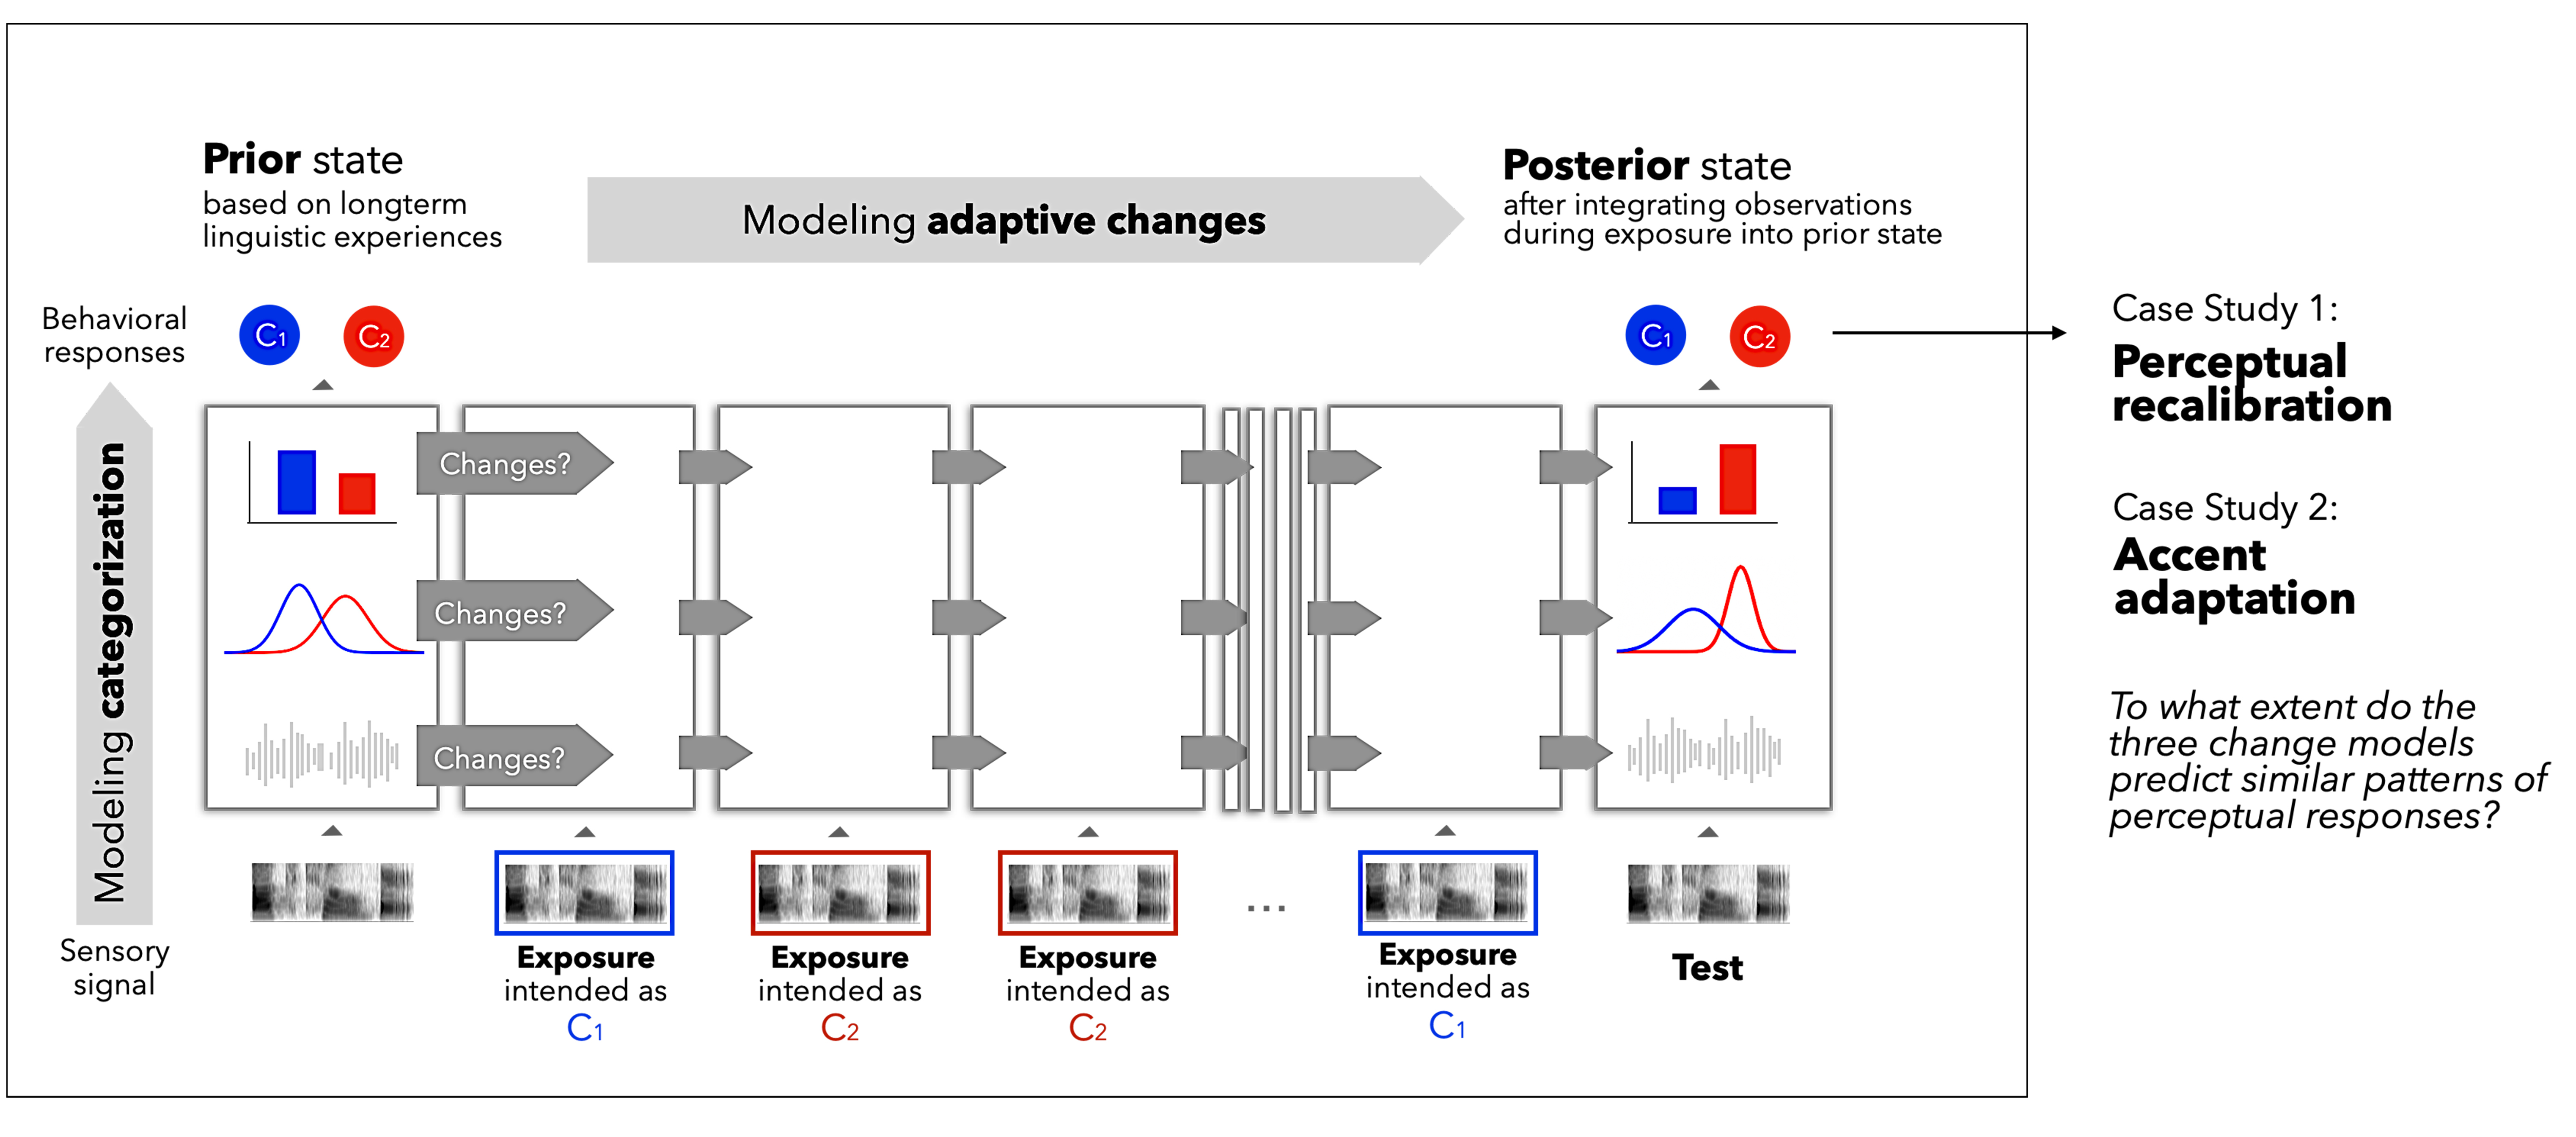
\includegraphics[width=.99\columnwidth]{../figures/diagrams/overview-of-changes.png}
\caption{Overview of the approach for the present study. Experiments on the effect of recent exposure on subsequent speech perception tend to involve two phases. An exposure phase manipulates the statistics of the speech input, typically between participants. A test phase---typically identical across participants---assesses the effects of those manipulations on the subsequent interpretation of speech input. We seek to understand what type of exposure effects each of the three mechanisms in Figure \ref{fig:overview} can explain. To this end, we specify both a) a {\em processing model}---specifically, a {\em categorization model}---that describes the interpretation of speech input at any given moment (vertical information flow) and b) {\em change models} for all three mechanisms that describe how these parts of the categorization model change as a function of exposure (horizontal information flow). We then use the different change models to compare the predicted consequences of changes to normalization, representations, or response biases.}\label{fig:overview-change}
\end{center}
\end{figure}

\hypertarget{the-categorization-model}{%
\subsection{The categorization model}\label{the-categorization-model}}

For the present purpose, we can think of the mapping from acoustic inputs to categorization responses as involving at least the three processes illustrated in Figure \ref{fig:model-perceptual-decision-making}. By presenting these processes as three different steps, we do not mean to imply that they are discrete, information encapsulated processes: ASP is agnostic as to whether and how the three mechanisms may interact with, or provide feedback to, each other during processing. We also emphasize that each of the three processes might in turn consist of several components that we abstract over here \autocite[e.g., multiple different levels of normalization, cf.~discussion in][]{barreda2020}.

\begin{figure}[h]
\begin{center}
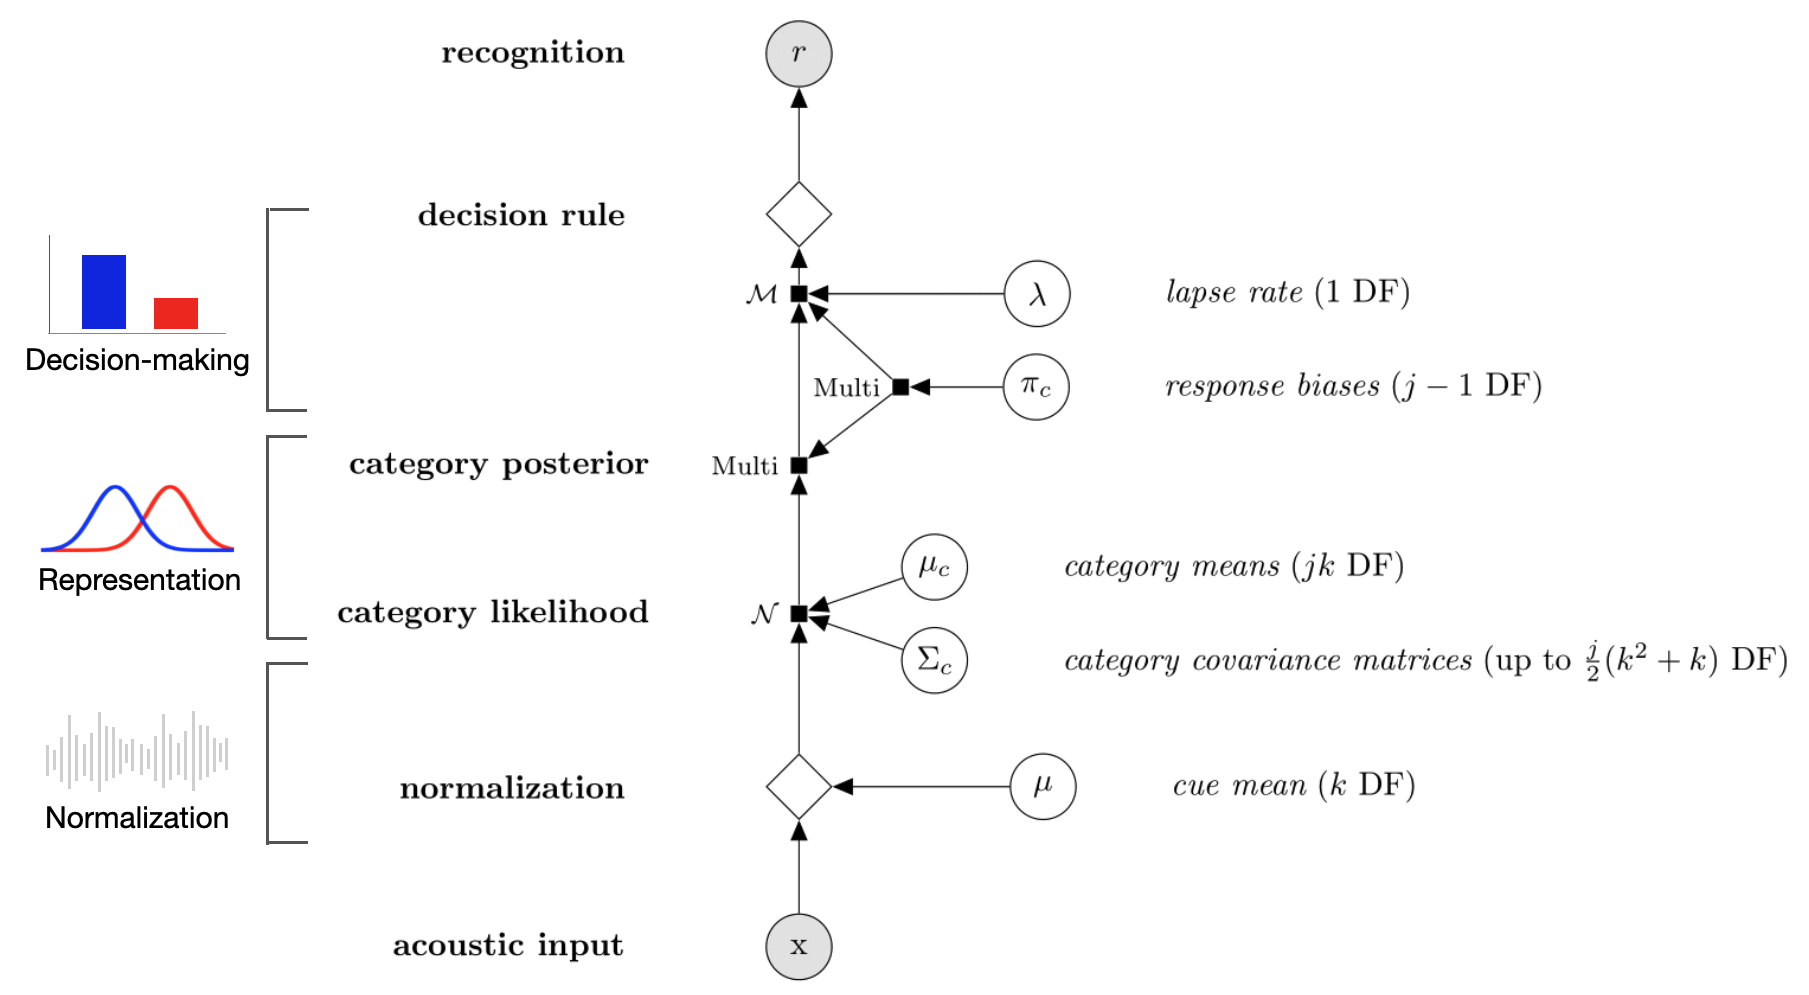
\includegraphics[width=.9\columnwidth]{../figures/diagrams/graphical-model.png}
  \caption{Graphical model of a simplified general {\em categorization model} for $J$-AFC alternative-choice tasks (e.g., vowel categorization, word transcription, etc.) over a $K$-dimensional phonetic input. The left-hand side links the components and parameters in the model to the three mechanism introduced in Figure \ref{fig:overview}. Filled gray circles represent variables the researcher can observe. Empty circles represent latent variables that are not observable. Diamonds represent variable-free processes. Only variables that we consider as being potentially affected by recent exposure are shown (see text for additional detail). Parentheses describe the number of degrees of freedom (DF) introduced by each parameter. In practice, many of these DFs can be fixed based on phonetic databases and/or previous perception experiments (see text for details). Squares are annotated with the distributions resulting at that level of the model: $\mathcal{N}$(ormal), Multi(nomial), and $\mathcal{M}$(ixture) distributions. For 2AFC tasks, all multinomial distributions simplify to Bin(omial) distributions.} \label{fig:model-perceptual-decision-making}
\end{center}
\end{figure}

\hypertarget{sec:normalization}{%
\subsubsection{`Pre-linguistic' auditory processes: signal transformations and normalization}\label{sec:normalization}}

The first step in our categorization model maps the acoustic input onto perceptual features. These perceptual features are the outcome of low-level signal transformations and normalization processes. Experiments on the perception of stimulus similarity suggest that the human brain represents frequency information logarithmically \autocite{greenwood1961}. This is captured by, for example, the Mel \autocite{stevens1937}, Bark \autocite{zwicker1961}, and ERB \autocite{moore-glasberg1983} transformations. Such logarithm-transformed spectral cues have been found to provide a better fit against human categorization responses than features based on raw frequencies \autocite{hoffmanbion-escudero2007,kleinschmidt2019,richter2017}. The case studies we present below model perception for a phonological contrast that depends on both temporal and spectral cues. For the spectral cue, we use Mel-transformed frequencies.

Many accounts of normalization assume further transformation of the acoustic input based either on other concurrently occurring acoustic properties (intrinsic normalization) or on the overall distribution of the acoustic input itself \autocites[extrinsic normalization, for review, see][]{weatherholtz-jaeger2016,clopper2009}. For example, some of the most influential normalization accounts for vowel formants either center \autocite[e.g.,][]{nearey1989} or both center and standardize formants based on the mean and standard deviation of the talker's formants \autocite[e.g.,][]{lobanov1971}. These transformations can remove a substantial amount of cross-talker variability in vowel realization \autocites[e.g.,][]{hoffmanbion-escudero2007,nearey1989,persson-jaeger2023}[for a particularly insightful review, see][]{barreda2020}. Importantly, models based on transformed formants provide a better fit against human vowel categorization than models based on untransformed cues \autocites[e.g.,][]{persson-jaeger2022,richter2017}, and there is evidence that this particularly true for centered log-transformed formants \autocite[i.e., Nearey's uniform scaling approach,][]{barreda2021}.

The case studies we present below employ a general model of normalization that can be applied to any type of phonological contrast \autocites[C-CuRE,][]{cole2010,mcmurray-jongman2011}. C-CuRE stands for ``computing cues relative to expectations''. Similar to some accounts of vowel normalization, C-CuRE centers cues by subtracting the (expected) mean for that cue in the current context (\(\mu\) in Figure \ref{fig:model-perceptual-decision-making}). C-CuRE has been found effective in accounting for cross-talker differences as well as effects of surrounding phonological context, improving the ability to predict human responses compared to a model without any normalization \autocites{mcmurray-jongman2011}[see also][]{apfelbaum-mcmurray2015,crinnion2020,kleinschmidt2020,mcmurray-jongman2016,xie2021cognition}. Figure \ref{fig:demonstrate-normalization} visualizes the effects of C-CuRE normalization on the marginal distributions of f0 and VOT to word-initial stop voicing in US English (e.g., /b/ vs.~/p/ in \emph{bin} vs.~\emph{pin}). The specific procedure is described in the SI (\ref{sec:SI-chodroff}). We use these normalized data throughout the remainder of this study, including the two case studies. That is, our case studies assume that listeners' \emph{long-term} expectations are based on talker-normalized cues (while investigating how normalization \emph{during the initial exposure} to an unfamiliar talker affects perception). The qualitative findings of our studies do not, however, depend on this assumption.



\begin{figure}

{\centering \includegraphics{../figures/knitted/demonstrate-normalization-1} 

}

\caption{Effects of applying C-CuRE normalization to productions of word-initial stop voicing in US English (e.g., \emph{bin} vs.~\emph{pin}). \textbf{Panel A:} unnormalized VOT and f0 of 40,459 stop productions from \textcite{chodroff-wilson2018}. VOT is the primary cue to this voicing contrast for L1 US English, and f0 is known to be a secondary cue. The data exhibit clear evidence of multimodality along both VOT and f0. \textbf{Panel B:} the same productions but after C-CuRE normalization has been applied to remove talker-specific variability. Compared to unnormalized data, the C-CuRE normalized data exhibits reduced variability and reduced evidence of multimodality (the remaining low-f0 outliers in the Panel B are the result of creaky voice and measurement errors like pitch-halving, see SI \ref{sec:SI-chodroff}).}\label{fig:demonstrate-normalization}
\end{figure}

Beyond signal transformations and normalization, the stimulus observed by a listener is also affected by external/environmental or internal/perceptual noise (not shown in Figure \ref{fig:demonstrate-normalization}). This means that even the same exact acoustic stimulus does not necessarily result in the same percept \autocites{leonard2016}[p.~148]{nearey-hogan1986}{schuerman2022}. The integration of internal noise into models of speech perception has been shown to explain otherwise puzzling differences in the perception and recognition of different types of phonological contrasts \autocites[e.g.,][]{feldman2009,kronrod2016}. Although not critical for the present purpose, we incorporate perceptual noise into ASP also because it results in more human-like (less steep) categorization functions. This noise is held constant across all case studies presented below, set to the values obtained by Kronrod and colleagues in their study of the L1-US English listeners' perception of word initial stop voicing \autocite*[\(\sigma^2_{noise, VOT}=80 msec^2\), \(\sigma^2_{noise, spectral}=878 Mel^2\)]{kronrod2016}.\footnote{Internal noise could affect processes at any level of Figure \ref{fig:demonstrate-normalization}, including the input to normalization, its output, or both. For normalization that is limited to linear transformations---such as centering (as in C-CuRE) and standardization--these possibilities are mathematically identical. In our case studies, we add internal noise prior to normalization, and do not add external noise (doing so would not affect the qualitative results). For an example of how to model external noise, see Burchill \autocite*[Chapter 3]{burchill2023}.}

\hypertarget{sec:representations}{%
\subsubsection{Category representations: from perceptual features to linguistic categories}\label{sec:representations}}

The output of normalization is the input to the mapping onto linguistic categories. All major theories of speech perception agree that this involves implicit knowledge of the distributional realization of linguistic categories---i.e., the distribution of acoustic or phonetic cues that are observed across instances of the category. In analytic models, this mapping is typically described by the \emph{category likelihood} that is learned from previous inputs \autocites[e.g., in the neighborhood activation model,][]{luce-pisoni1998}[shortlist B,][]{norris-mcqueen2008}[and other Bayesian inference models,][]{clayards2008,feldman2009,kleinschmidt-jaeger2015}. In exemplar models and related theories, the same mapping is achieved by storing previously experienced inputs as exemplars \autocites[e.g.,][]{johnson2006,pierrehumbert2001,wedel2006} or episodic traces \autocite{goldinger1996} that subsequent inputs are compared to during recognition \autocite[e.g., by means of \(k\)-nearest neighbor algorithms,][]{fix-hodges1989}. In connectionist and deep neural network models, the same probabilistic mapping is achieved through latent structure in the network that is learned from previous input \autocite{mcclelland-elman1986,magnuson2020}. Although the specific nature of these representations continues to be a matter of debate, all of these theories share the assumption that there is a probabilistic mapping between perceptual cues and linguistic categories \autocite[see also][ on the close computational relation between exemplar and Bayesian inference models]{shi2010} and that perception involves implicit knowledge of this probabilistic mapping.

Here we employ an analytic characterization of category likelihoods. Specifically, we adopt a simplifying assumption commonly made in research on speech perception \autocite{clayards2008,feldman2009,kleinschmidt-jaeger2015,norris-mcqueen2008} and automatic speech recognition \autocite{jurafsky-martin2000} that the cue distributions for each category follow a multivariate Gaussian distribution. In Figure \ref{fig:model-perceptual-decision-making}, this is indicated through the two parameters that are sufficient to specify each multivariate Gaussian (the category means \(\mu_c\) and the category covariance matrices \(\Sigma_c\)).\footnote{\label{fn:alternative-representational-changes} The assumption of multivariate Gaussian categories strikes a compromise between two common alternatives. A representationally less complex proposal introduces an independence assumption and describes linguistic categories as a combination of \emph{independent uni}variate Gaussians for each cue dimension. The likelihoods from the univariate Gaussians is then combined through a cue integration model. This substantially reduces the degrees of freedom that need to be estimated---both for learners/listeners and the researcher \autocite[see][]{toscano-mcmurray2010}. A representationally more complex alternative dispenses with the Gaussian assumption and instead assumes that listeners store all previously experienced exemplars \autocite[or some pruned set of exemplars,][]{pierrehumbert2001}. This allows for more accurate (non-parametric) representations of previous experience but also introduces many additional degrees of freedom--both for learners/listeners and the researcher \autocite[for discussion, see][]{apfelbaum-mcmurray2015}. We expect the big picture conclusions we draw below to be largely independent of the specific model of category representations.} Bivariate Gaussian categories fit to the data from \textcite{chodroff-wilson2018} are shown in Figure \ref{fig:show-representations-plots}. The bottom row of the same figure shows the predicted categorization functions over the VOT-f0 space, prior to considering additional aspects of decision-making that we discuss next.



\begin{figure}

{\centering \subfloat[Distributions for /b/ and /p/\label{fig:show-representations-plots-1}]{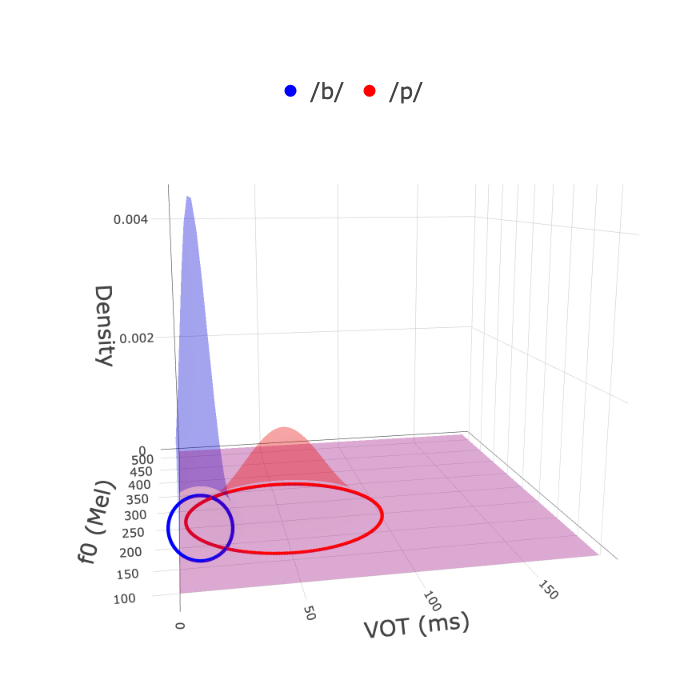
\includegraphics[width=0.33\linewidth,height=0.49\textheight]{../figures/plotly//p.3d.density.panel_1} }\subfloat[Distributions for /d/ and /t/\label{fig:show-representations-plots-2}]{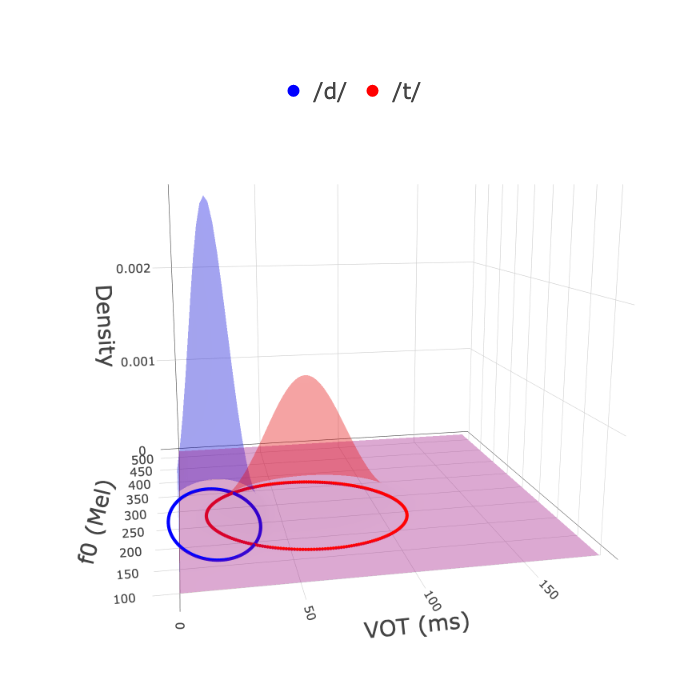
\includegraphics[width=0.33\linewidth,height=0.49\textheight]{../figures/plotly//p.3d.density.panel_2} }\subfloat[Distributions for /g/ and /k/\label{fig:show-representations-plots-3}]{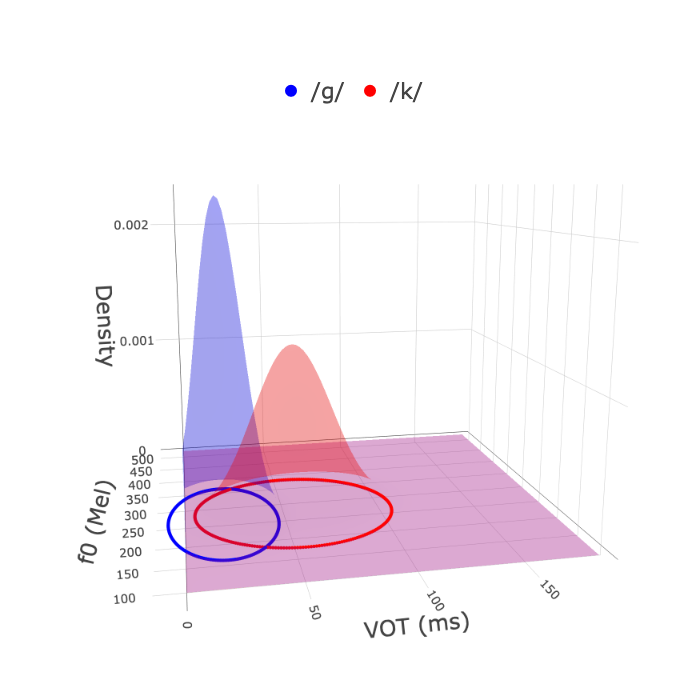
\includegraphics[width=0.33\linewidth,height=0.49\textheight]{../figures/plotly//p.3d.density.panel_3} }\newline\subfloat[Categorization for /b/-/p/\label{fig:show-representations-plots-4}]{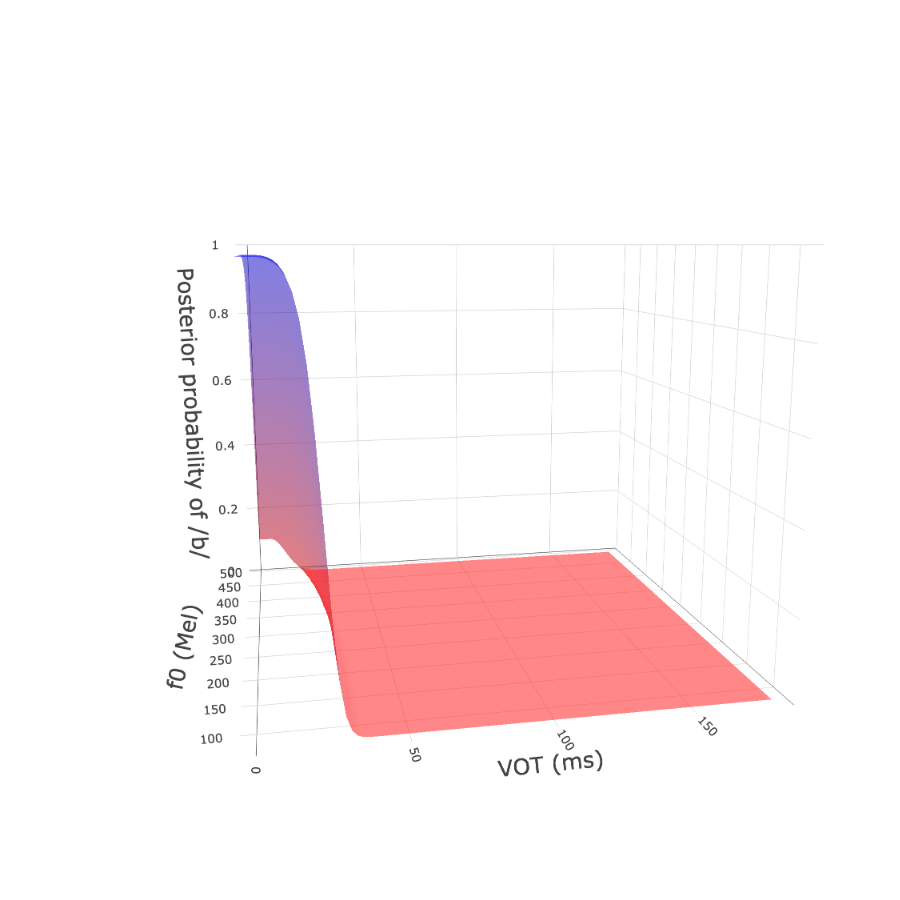
\includegraphics[width=0.33\linewidth,height=0.49\textheight]{../figures/plotly//p.3d.categorization.panel_1} }\subfloat[Categorization for /d/-/t/\label{fig:show-representations-plots-5}]{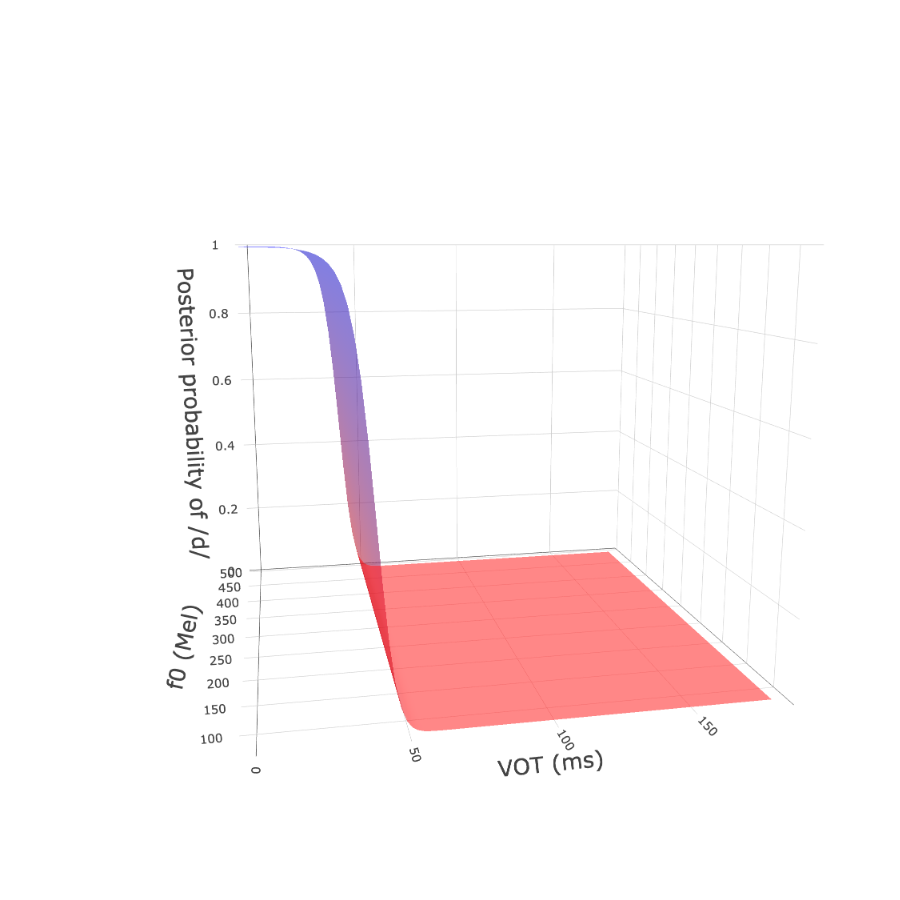
\includegraphics[width=0.33\linewidth,height=0.49\textheight]{../figures/plotly//p.3d.categorization.panel_2} }\subfloat[Categorization for /g/-/k/\label{fig:show-representations-plots-6}]{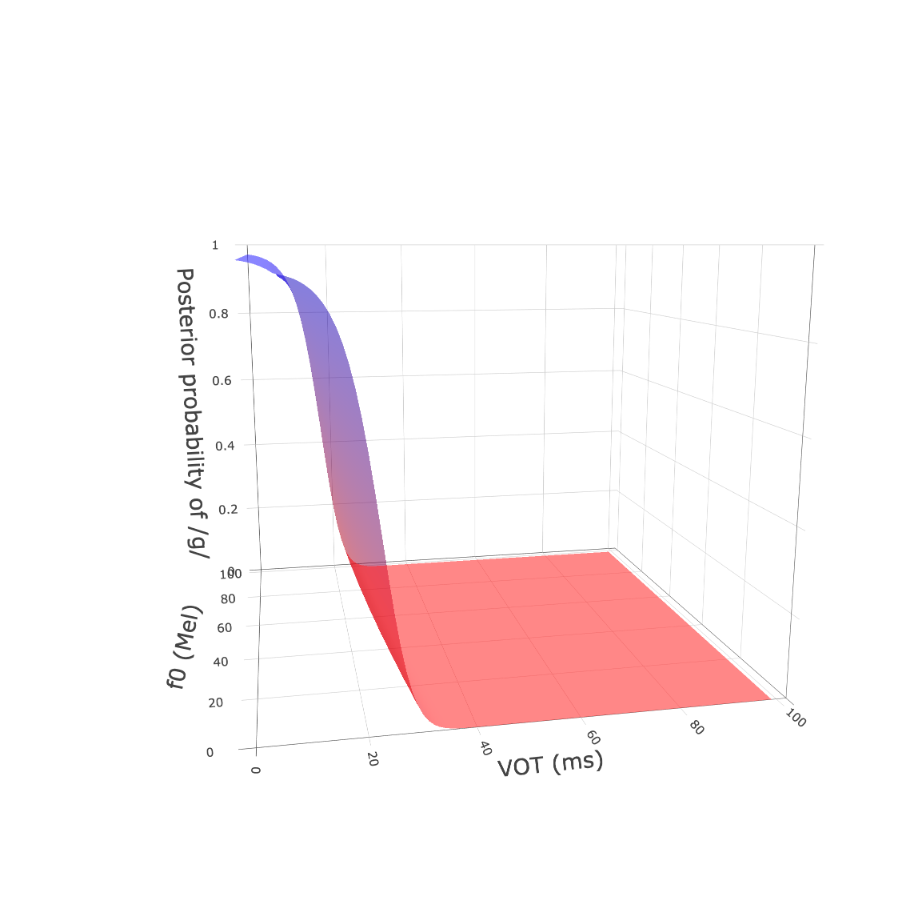
\includegraphics[width=0.33\linewidth,height=0.49\textheight]{../figures/plotly//p.3d.categorization.panel_3} }

}

\caption{Illustrating listeners' implicit category representations. \textbf{Top row:} Bivariate Gaussian category likelihoods learned from (fit to) the by-talker normalized cue distributions in Figure \ref{fig:demonstrate-normalization}B. Ellipses show 95\% probability mass. \textbf{Bottom row:} Categorization functions that would result from these category likelihoods prior to taking into account other effects on decision-making (see Figure \ref{fig:show-lapse-bias-demonstration-plots} in the next section).}\label{fig:show-representations-plots}
\end{figure}

\hypertarget{post-perceptual-decision-making-incorporating-priors-response-biases-and-attentional-lapses}{%
\subsubsection{Post-perceptual decision-making: incorporating priors, response biases, and attentional lapses}\label{post-perceptual-decision-making-incorporating-priors-response-biases-and-attentional-lapses}}

The third and final step in our categorization model takes the output of the second step and derives a decision/recognition.\footnote{This step can be split further into \emph{recognition} of the category and post-recognition processes that affect the behavioral \emph{response}. For the present purpose, we group these processes together. Similarly, some models of perceptual decision-making distinguish between \emph{decision thresholds} (the amount of evidence necessary before a decision is being made) and \emph{decision biases} \autocites[stimulus-independent effects on the activation or probability of a response option,][]{clarkedavidson2008,venezia2012}. For the present purpose, these two have essentially identical effects.} This includes the integration of information about the prior probability of a category \(c\) in the current context, \(p(c | context)\), including well-documented effects of, e.g., phonotactic, prosodic, lexical/semantic, visual and sentential/discourse contexts \autocite[for a great concise review, see][]{winn2018}. In Bayesian ideal observer models, this integration takes place according to Bayes theorem, yielding an estimate of each category's posterior probability \autocites[e.g.,][]{luce-pisoni1998,norris-mcqueen2008}. Alternative computational approaches can introduce additional degrees of freedom, for example, by allowing non-optimal weighting of priors and category likelihoods. As our goal here is to arrive at the simplest possible model, we follow the approach taken in ideal observers:

\begin{equation}\label{eq:posterior-probability}
\begin{split}
p(c | input) & = \frac{p(input | c) p(c)}{\Sigma_i p(input | c_i) p(c_i)} \\
                    & = \frac{\mathcal{N}\!(input | \mu_c, \Sigma_c) p(c)}{\Sigma_i \mathcal{N}\!(input | \mu_{c_i}, \Sigma_{c_i}) p(c_i)}
\end{split}
\end{equation}

where the second row substitutes the Gaussian category likelihoods assumed in the previous section into the equation. In Bayesian models, \(p(c_i)\) is generally assumed to reflect a rational estimate based on either the relative frequency of the category in this type of context in listeners' longterm experience or an estimate based on the expectations about the present context. The latter allows for the integration of \emph{response biases} that go beyond capturing the relative frequency of categories in previous experience. In an experiment with a 2AFC task, for example, participants might expect both response options to occur about equally often. This might lead participants to adjust response biases based on the sequence of most recently observed categories. The simplified model in Figure \ref{fig:model-perceptual-decision-making} captures these response biases---regardless of whether they reflect priors based on the relative frequency of categories, meta-reasoning about the structure of experiments, or other factors---through the parameters \(\pi_{c}\). For a \(J\)-way categorical outcome, this introduces \(J-1\) degrees of freedom (since \(\Sigma_i \pi_{c_i} = 1\)) that cannot be independently estimated from phonetically annotated databases. These parameters can, however, often be set based on assumptions about the current task as well as on the extent to which prior expectations about natural language transfer to this task. For example, standard experimental designs provide participants with ample evidence that prior expectations based on the relative frequency of lexical items in natural language use do \emph{not} transfer to the experiment \autocite[cf.][]{jaeger2010}. In such contexts, participants might quickly come to adjust their expectations and employ uniform response biases.

In addition to response biases, the categorization model in Figure \ref{fig:model-perceptual-decision-making} includes the possibility that listeners sometimes respond \emph{in}dependent of the stimulus. As we will show below, this is a critical addition that affects what types of behavioral changes can be explained by changes in decision biases. Stimulus-independent responses can occur, for example, because of attentional lapses. On such occasions, the response is only influenced by the response biases. Lapsing models \emph{without} consideration of response biases have previously been used in some analyses of exposure effect on speech perception \autocite{clayards2008,mcmurray-jongman2011,kleinschmidt-jaeger2016cogsci}. For the present purpose, we further assume that these response biases on lapsing trials are identical to the response biases on non-lapsing trials. Assuming equal priors for all alternative categories, this yields the following simplified model of the joint effect of attentional lapses and response biases, where \(\lambda\) is lapse rate---the probability of lapsing:\footnote{Readers familiar with psychometric models might recognize the close relation between Equation \eqref{eq:posterior-probability-lapse} and the standard psychometric model in \textcite{wichmann-hill2001}: \(\gamma + (1-\gamma-\lambda) F(stimulus | \alpha, \beta)\). In the Wichmann and Hill model, \(\gamma\) describes the floor and \(1-\lambda\) describes the ceiling probability. In Equation \eqref{eq:posterior-probability-lapse}, \(\lambda\) is the lapse rate and \(\pi_c\) determines how the lapses (and non-lapses) are affected by response biases, resulting in a floor of \(\lambda \pi_c\) and a ceiling of \(1 - \lambda(1 - \pi_c)\). For the special case of two Gaussian categories with identical variance along a unidimensional cue continuum, Equation \eqref{eq:posterior-probability-lapse} can be described by Wichmann and Hill's psychometric model if the perceptual model \(F\) is set to be a logistic function with appropriate choice of its threshold \(\alpha\) and slope \(\beta\) \autocite[cf.][p.~200]{kleinschmidt-jaeger2015}. For unequal variances and/or additional cue dimensions, additional \(\beta\)s are required.}

\begin{equation}\label{eq:posterior-probability-lapse}
p(c | input) = (1 - \lambda) \frac{\mathcal{N}\!\left( input | \mu_c, \Sigma_c \right) \pi_c}{\Sigma_i \mathcal{N}\!\left( input | \mu_{c_i}, \Sigma_{c_i} \right) \pi_{c_i}} + \lambda \frac{\pi_c}{\Sigma_i \pi_{c_i}}
\end{equation}

In Figure \ref{fig:model-perceptual-decision-making}, the fact that response bias affects listeners' responses in both lapsing and non-lapsing trials is indicated by the two arrows leaving from \(\pi_c\). Figure \ref{fig:show-lapse-bias-demonstration-plots} visualizes the effects of the two parameters \(\lambda\) and \(\pi_c\) for a 2AFC categorization task.



\begin{figure}

\subfloat[$\lambda$ = 0, $\pi_{/d/}=.5$\label{fig:show-lapse-bias-demonstration-plots-1}]{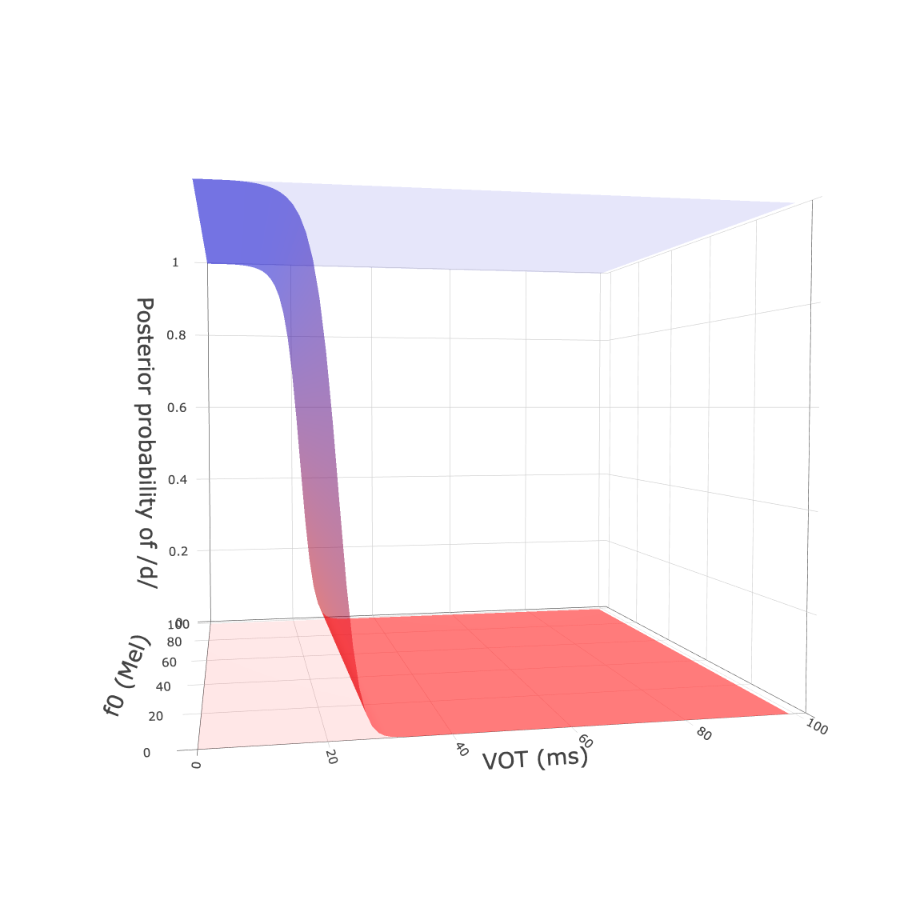
\includegraphics[width=0.33\linewidth,height=0.49\textheight]{../figures/plotly//p.3d.categorization.panel_lambda=1} }\subfloat[$\lambda$ = .2,  $\pi_{/d/}=.5$\label{fig:show-lapse-bias-demonstration-plots-2}]{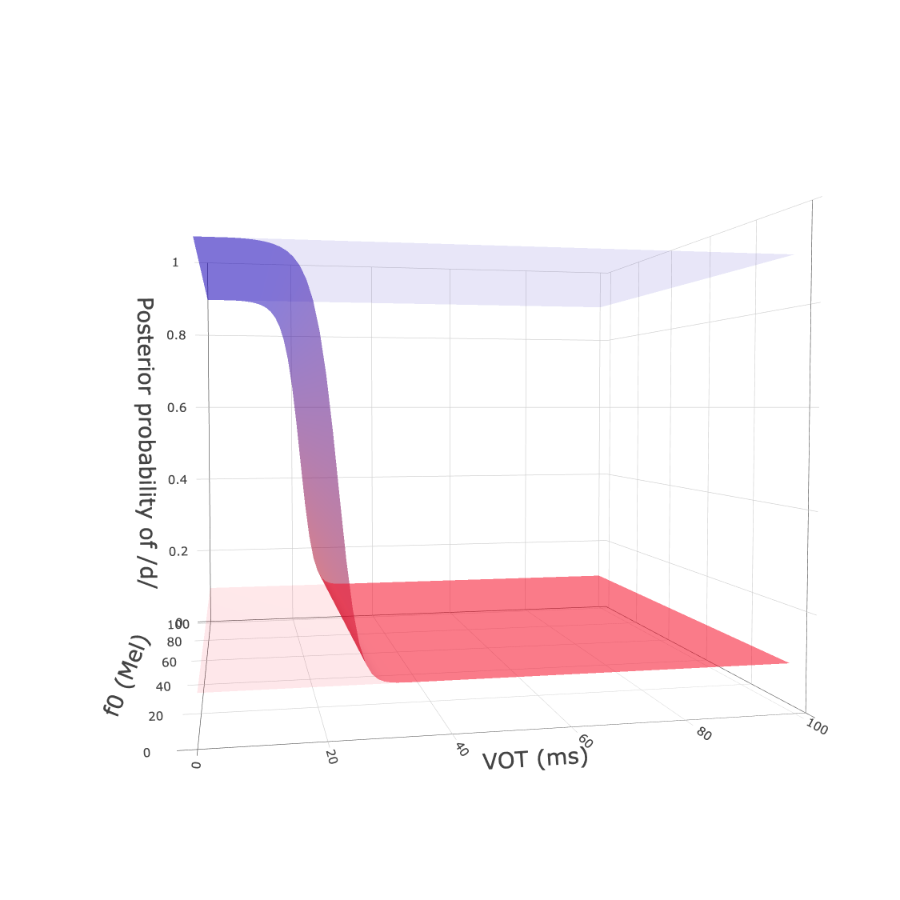
\includegraphics[width=0.33\linewidth,height=0.49\textheight]{../figures/plotly//p.3d.categorization.panel_lambda=2} }\newline\subfloat[$\lambda$ = .2, $\pi_{/d/}=.1$\label{fig:show-lapse-bias-demonstration-plots-3}]{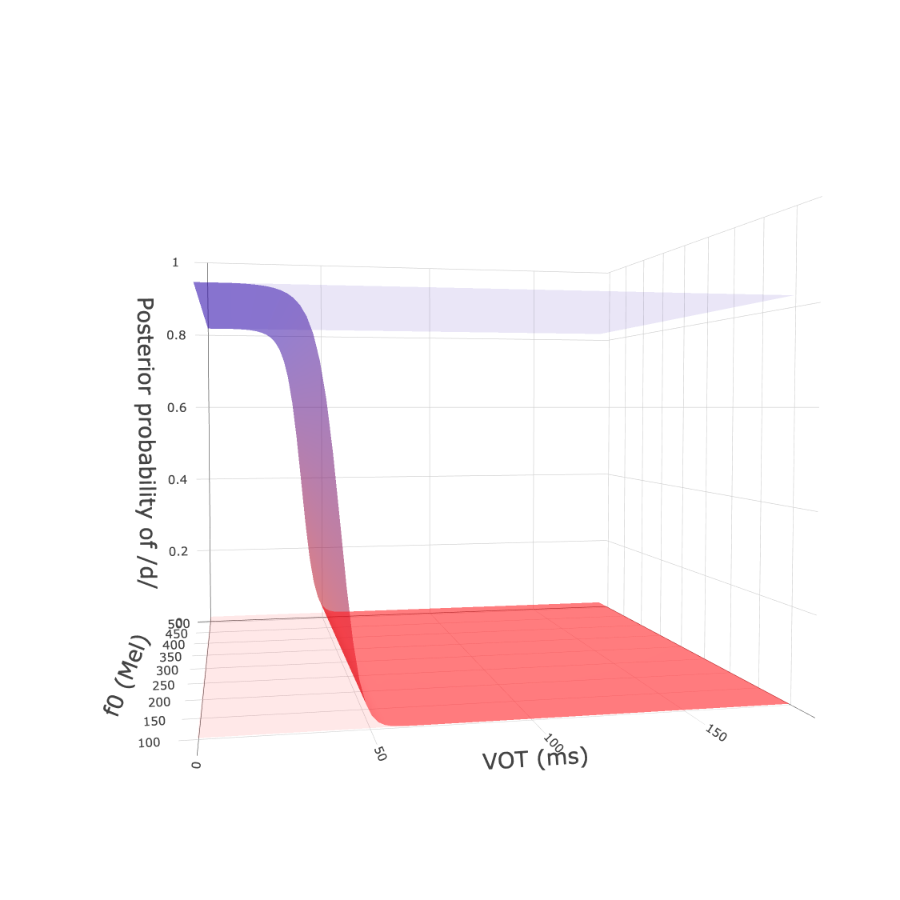
\includegraphics[width=0.33\linewidth,height=0.49\textheight]{../figures/plotly//p.3d.categorization.panel_pi=1} }\subfloat[$\lambda$ = .2, $\pi_{/d/}=.9$\label{fig:show-lapse-bias-demonstration-plots-4}]{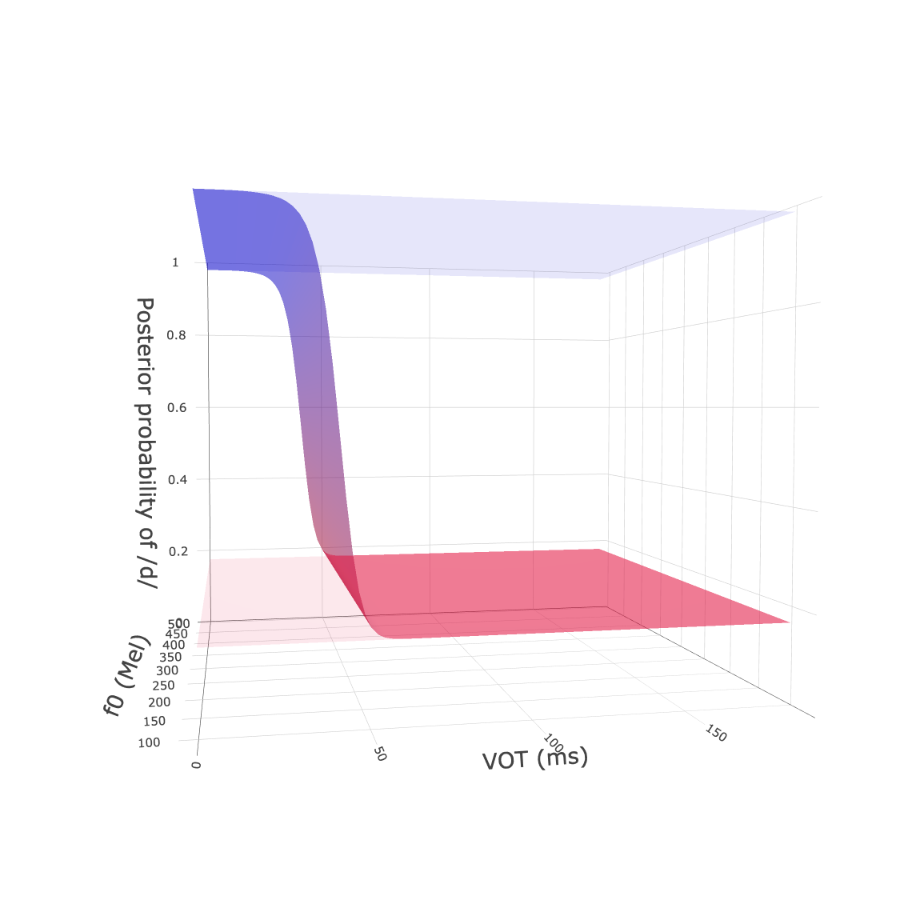
\includegraphics[width=0.33\linewidth,height=0.49\textheight]{../figures/plotly//p.3d.categorization.panel_pi=2} }\hfill{}

\caption{Illustrating the effects of \(\lambda\) and \(\pi_c\) on the posterior probability of /d/, using the two bivariate Gaussian categories of /d/ and /t/ shown in Figure \ref{fig:show-representations-plots}b. The colored planes indicate the ceiling and flooring levels of posterior probability of /d/. Panel a) here is identical to Panel e) in Figure \ref{fig:show-representations-plots},with \(\lambda\) = 0 and \(\pi_{/d/}=.5\). \textbf{Top panel:} Differences in lapse rate \(\lambda\) for a uniform bias of \(\pi_{/d/}=.5\). As the lapse rate increases, the ceiling and flooring responses at the end points change while the categorization slope remains the same. \textbf{Bottom panel:} Differences in bias \(\pi_{/d/}\) when the lapse rate \(\lambda\) = .2. As the bias towards /d/ changes from 0.1 to 0.9, the categorization surface shifts upwards and to the right, resulting in more /d/ responses across the phonetic space.}\label{fig:show-lapse-bias-demonstration-plots}
\end{figure}

The final part of ASP's categorization model is the decision rule that takes the posterior in Equation \eqref{eq:posterior-probability-lapse} as input and returns a response. Here, we follow a common assumption in research in speech perception and employ Luce's choice rule \autocites{luce1959}[for a comparison of decision rules, see][]{massaro-friedman1990}. Under this decision rule, the predicted distribution of responses is identical to the posterior in Equation \eqref{eq:posterior-probability-lapse}. For example, in a 2AFC categorization task, a posterior probability of .3 for /d/ and .7 for /t/ would result in a /d/-response with .3 probability or a /t/-response with .7 probability.

This completes the description of the categorization model in Figure \ref{fig:model-perceptual-decision-making}. For any parameterization of \(\lambda\), \(\pi_c\), \(\mu_c\), \(\Sigma_c\), and \(\mu\), this model takes acoustic stimuli as input and returns predictions about the expected response distribution (e.g., 30\% /d/-responses and 70\% /t/-responses). In practice, all but one of these parameters (the lapse rate \(\lambda\)) can either be independently estimated from phonetically annotated databases (\(\mu_c\), \(\Sigma_c\), and \(\mu\)) or assumed to have certain values (e.g., uniform response biases \(\pi_c\)), leaving a single parameter that must be estimated from perceptual data.

\hypertarget{sec:change-models}{%
\subsection{The change models (`adaptation'/`learning')}\label{sec:change-models}}

Next, we extend this model to capture \emph{changes} at any of the three mechanistic levels. That is, we specify \emph{change models} that describe how \(\pi_c\), \(\mu_c\), \(\Sigma_c\), and \(\mu\) can change with exposure. It is these change models that make it possible to use ASP to derive predictions for human responses following exposure---for example, during the test phase of an experiment on perceptual recalibration or accent adaptation (see Figure \ref{fig:overview-change}). Each of the three change models introduces at least one new parameter. These parameter determine the speed of adaptation (similar to learning rates), and must be estimated from perceptual data.

As anticipated in the introduction, the three change models differ in their computational and representational parsimony---i.e., in the number of parameters that listeners (and researchers) need to infer as well as the amount of information that listeners are assumed to keep in memory.

\hypertarget{sec:change-normalization}{%
\subsubsection{\texorpdfstring{Modeling \emph{changes} in normalization}{Modeling changes in normalization}}\label{sec:change-normalization}}

\begin{figure}
\centering
  \tikz{ %
    \node[obs] (x_in) {x} ; %
    \node[det, above=of x_in] (x_prime) {} ; %
    \node[above=of x_prime] (dots) {$\vdots$} ; %
    \node[det, right=of x_prime] (mu_n) {$\mu_N$} ; %
    \node[obs, right=of mu_n, yshift=-.75cm] (xbar) {$\bar{x}$} ; %
    \node[right=of xbar] (xbar_description) {{\em cue mean observed from unfamiliar talker}} ;
    \node[obs, below=of xbar, yshift=.5cm] (n) {$N$} ; %
    \node[right=of n] (n_description) {{\em number of observations from unfamiliar talker}} ;
    \node[latent, right=of mu_n, yshift=.75cm] (mu_0) {$\mu_0$} ; %
    \node[right=of mu_0] (mu_0_description) {{\em prior beliefs about cue mean} ($k$ DF)} ;
    \node[latent, above=of mu_0, yshift=-.5cm] (kappa_0) {$\kappa_0$} ; %
    \node[right=of kappa_0] (kappa_0_description) {{\em strength of prior beliefs about cue mean} (1 DF)} ;
    \edge {x_in} {x_prime} ; %
    \edge {x_prime} {dots} ; %
    \edge {mu_n} {x_prime} ; %
    \edge {mu_0} {mu_n} ; %
    \edge {kappa_0} {mu_n} ; %
    \edge {xbar} {mu_n} ; %
    \edge {n} {mu_n} ; %
}
\caption{Graphical representation of Equation \ref{eq:normalization-change}, describing how normalization changes with exposure. $\mu_N$ here substitutes $\mu$ in Figure \ref{fig:model-perceptual-decision-making}, removing those DFs from the categorization model). While we mark the prior cue mean $\mu_0$ as a latent variable, it can be estimated from phonetic databases (as we do in  Case Studies 1 and 2), leaving $\kappa_0$ as the only DF for this change model.\label{fig:graphical-model-changes-normalization}}
\end{figure}

C-CuRE and most other models of normalization assume that the theoretical quantities employed in normalization---for C-CuRE, the means of all cues---are \emph{known} to the listeners \autocites[e.g.,][]{apfelbaum-mcmurray2015,mcmurray-jongman2011}. However, listeners must somehow \emph{infer} these quantities from the observed inputs \autocites[see also][]{barreda2012,magnuson-nusbaum2007,weatherholtz-jaeger2016}. For example, in the types of experiments we consider below, listeners need to \emph{infer} the unfamiliar talker's cue means from the inputs observed during exposure. At the beginning of exposure, the best estimates of the cue means for the unfamiliar talker are the mean expected based on listeners' longterm experience with various different talkers (\(\mu_0\)). With increasing exposure to the unfamiliar talker, listeners can update their estimates of the talker's cue means based on the input. ASP thus expands C-CuRE with a linking hypothesis that describes how listeners update their estimates of the unknown mean.

Some proposals for such functions include moving-window algorithms that estimate the mean as the sample mean over a finite number of the most recent observations \autocite{lee2002,zhang-peng2021}. Here, we model listeners' estimate of the talker-specific cue mean \(\mu_N\) after \(N\) observations from that talker as simple linear interpolation between the cue mean observed in previous longterm experience (\(\mu_0\)) and the mean observed in the sample observed from the unfamiliar talker (\(\bar{x}\)). This approach has the advantage that listeners can draw on prior experience when they do not yet have much (or any) data from an unfamiliar talker. They can then update the inferred cue mean as they observe further data from the talker \autocite[see discussion of the flexibility-stability trade-off in][p.~178-182]{kleinschmidt-jaeger2015}:

\begin{equation}\label{eq:normalization-change}
\mu_N = \frac{1}{\kappa_0 + N} \left( \kappa_0 \mu_0 + N \bar{x} \right) = \frac{\kappa_0}{\kappa_0 + N} \mu_0 + \frac{N}{\kappa_0 + N}\bar{x}
\end{equation}

Figure \ref{fig:graphical-model-changes-normalization} expresses Equation \eqref{eq:normalization-change} as a graphical model. The two parameters describing the input from the unfamiliar talker, \(N\) and \(\bar{x}\), are determined by the exposure data used in the experiment (the estimation of the cue means, \(\bar{x}\) requires that the exposure stimuli are phonetically annotated). \(\mu_0\) can be estimated from sufficiently large phonetically annotated databases of speech, essentially assuming that listeners have learned the overall cue means across talkers from previously experienced speech input. This is what we did to create Figure \ref{fig:demonstrate-normalization}, and it is what we assume in the remainder of this study. At the minimum, this leaves only one degree of freedom that is not independently determined: the relative weight of previous experience compared to the input received from the talker so far (\(\kappa_0\)). This is the parameter we vary in the case studies presented below to illustrate the types of results that can be explained through changes in normalization due to recent exposure.

One important characteristic of normalization that we will return to in the general discussion is that it applies to cues \emph{regardless of the category an observation is inferred to originate from}. On the one hand, this makes normalization potentially very efficient, by considering \emph{all} available information about a cue, rather than just observations of a specific category \autocite{apfelbaum-mcmurray2015}. On the other hand, this limits what types of changes in the mapping from cues to categories normalization can account for.

\hypertarget{sec:ideal-adaptor}{%
\subsubsection{\texorpdfstring{Modeling \emph{changes} in category representations}{Modeling changes in category representations}}\label{sec:ideal-adaptor}}

Just like normalization requires inference of \emph{overall} cue statistics (e.g., the overall mean of a cue), learning of category representations requires inferences of \emph{category-specific} cue statistics (e.g., the category mean and covariance). Changes in representations can thus be understood as the process of inferring the talker's category likelihood function, the distribution of phonetic cues conditional on the category. A theory of this inference process---the ideal adaptor---is introduced in \textcite{kleinschmidt-jaeger2015}. Bayesian belief-updating models based on the ideal adaptor framework have been shown to provide a good qualitative and quantitative fit against human responses in experiments on perceptual recalibration \autocites{kleinschmidt-jaeger2011,kleinschmidt-jaeger2012}[for closely related models, see][]{xie2021cognition}, selective adaptation \autocite{kleinschmidt-jaeger2016pbr}, unsupervised or semi-supervised distributional learning \autocites[e.g.,][]{kim2020,kleinschmidt-jaeger2016cogsci,theodore-monto2019}[for closely related model, see][]{bejjanki2011,clayards2008}, and accent adaptation \autocites{hitczenko-feldman2016}[for a closely related model, see][]{tan2021}. In a MEG experiment, \textcite{sohoglu-davis2016} found that their predictive coding implementation of Bayesian belief-updating provided a good qualitative fit against changes in activation in the superior temporal gyrus following exposure to degraded speech \autocite[see also][]{davis-sohoglu2020}. To date, however, an explicit comparison with alternative types of change models---like normalization or changes in decision-making---continues to be lacking.

The Bayesian belief-updating model introduced in \textcite{kleinschmidt-jaeger2015} describes the inference of category means and category variances in ways that are conceptually similar to the type of interpolation we described in Equation \eqref{eq:normalization-change}, by combining knowledge based on previously experienced speech input \(\mathcal{D}_0\) with the observations made from the unfamiliar talker. The specific instance of the model we use here---belief-updating over a Normal-Inverse-Wishart (\(\mathcal{NW^{-1}}\)) prior---describes the uncertainty listeners have about the category means \(\mu_c\) and category covariance matrices \(\Sigma_c\) prior to any observations from an unfamiliar talker as a function of four variables \autocite[p.~132-3]{murphy2012}:

\begin{equation}\label{eq:niw-updating}
\begin{split}
p\left( \mu_c, \Sigma_c | \mathcal{D}_0 \right) & = \mathcal{NW}^{-1} \left( \mu_c, \Sigma_c | \mathrm{m}_{c,0}, \kappa_{c,0}, \nu_{c,0}, \mathrm{S}_{c,0} \right) \\
& = \mathcal{N}\left( \mu_c | \mathrm{m}_{c,0}, \frac{1}{\kappa_{c,0}} \Sigma_{c} \right) \times \mathcal{W}^{-1}\left( \Sigma_c | \mathrm{S}_{c,0}, \nu_{c,0} \right)
\end{split}
\end{equation}

The Normal part of the \(\mathcal{NW^{-1}}\) model describes the uncertainty about the category mean \(\mu_c\), the Inverse-Wishart part describes the uncertainty about the category covariance \(\Sigma_c\). For the former, \(\mathrm{m}_{c,0}\) is the mean of the normal distribution describing the uncertainty about the category mean \(\mu_c\), and \(\kappa_{c,0}\) indicates the extent to which listeners transfer their prior beliefs about the category mean to the present input. The larger \(\kappa_{c,0}\) is, the more certain listeners are about the category mean even prior to any observation, and the less their inferences about the talker's category mean will be influenced by observations from the talker. Put differently, larger \(\kappa_{c,0}\) predicts slower learning of changes in the category mean. Similarly, \(\mathrm{S}_{c,0}\) is the scale matrix of the Inverse-Wishart---having a conceptually similar function to the mean \(\mathrm{m}_{c,0}\) of the Normal distribution---and \(\nu_{c,0}\) indicates extent to which listeners transfer their prior beliefs about the category covariance to the present input. Just as larger \(\kappa_{c,0}\) predicts slower learning of changes in the category mean, larger \(\nu_{c,0}\) predicts slower learning of changes in the category covariances.

In practice, researchers can estimate the \(\mathrm{m}_{c,0}\)s and the \(\mathrm{S}_{c,0}\)s such that they yield the distribution of category means and covariances that would be expected given listeners' previous long-term experience (see SI, \ref{sec:SI-models-changes-in-representations}). This leaves two degrees of freedom to model changes in each category's likelihood, \(\kappa_{c,0}\) and \(\nu_{c,0}\). We further follow previous work to make the simplifying assumption that all categories have the same prior \(\kappa_{c,0}\) and \(\nu_{c,0}\) \autocite{kleinschmidt-jaeger2015,kleinschmidt-jaeger2016cogsci}, leaving just two degrees of freedom \emph{across} all categories to model changes in representations. These are the two parameters we vary in the case studies presented below to illustrate the types of results that can be explained through changes in representations. Figure \ref{fig:demonstrate-niw-prior-mu-sigma} demonstrates how \(\kappa_{c,0}\) and \(\nu_{c,0}\) affect the uncertainty about the category likelihoods for the simple case of univariate Gaussian categories along a single cue dimension (VOT). The case studies we present below employ bivariate Gaussian categories along f0 and VOT.



\begin{verbatim}
## $rows
## [1] 1.18110236220472null
## 
## $cols
## [1] 1.37795275590551null
## 
## $respect
## NULL
## 
## attr(,"class")
## [1] "forcedsize"
\end{verbatim}

\begin{figure}

{\centering \includegraphics{../figures/knitted/demonstrate-niw-prior-mu-sigma-1} 

}

\caption{Illustrating the effects of \(\kappa_{c,0}\) and \(\nu_{c,0}\) on the uncertainty about the category means \(\mu_c\) and variances \(\Sigma_c\) for univariate /d/ and /t/ categories along VOT. The four priors have identical expected category means (\(\mathbf{E}(\mu_{/d/}), \mathbf{E}(\mu_{/t/})\)) and variances (\(\mathbf{E}(\sigma_{/d/}), \mathbf{E}(\sigma_{/t/})\))---set to match the average of the C-CuRE normalized category means and covariance matrices obtained from the data in \textcite{chodroff-wilson2018}, and indicated by black points. The four priors differ, however, in their uncertainty about the category means and variances and thus in the changes they predict to occur when exposed to input from an unfamiliar talker. The more uncertain a listener is about the category means and variances of an unfamiliar talker (smaller \(\kappa_{c,0}\) and \(\nu_{c,0}\)), the quicker that listener will adjust their expectations based on the inputs observed from that talker (see Figures \ref{fig:demonstrate-changes-in-representations} and \ref{fig:demonstrate-changes-in-representations-b}). Density lines are drawn at \(10^{-3}\) to \(10^{-10}\) at powers of 10.}\label{fig:demonstrate-niw-prior-mu-sigma}
\end{figure}

\begin{figure}
\centering
  \tikz{ %
    \node (x_in) {$\vdots$} ; %
    \factor[above=of x_in] {x_prime} {left:$\mathcal{N}$} {} {}; %
    \node[above=of x_prime] (dots) {$\vdots$} ; %
    \node[det, right=of x_prime, yshift=2cm] (mu_n) {$\mu_{c,N}$} ; %
    \node[det, right=of x_prime, yshift=-2cm] (sigma_n) {$\Sigma_{c,N}$} ; %
    % Change model for mean
    \node[latent, right=of mu_n, yshift=.75cm] (m_0) {${\rm m}_{c,0}$} ; %
    \node[right=of m_0] (m_0_description) {{\em prior beliefs about category mean} ($jk$ DF)} ;
    \node[latent, above=of m_0, yshift=-.5cm] (kappa_0) {$\kappa_{c,0}$} ; %
    \node[right=of kappa_0] (kappa_0_description) {{\em strength of prior beliefs about category mean} (up to $j$ DF)} ;
    \node[obs, right=of mu_n, yshift=-.75cm] (xbar) {$\bar{x_c}$} ; %
    \node[right=of xbar] (xbar_description) {{\em category mean observed from unfamiliar talker}} ;
    \node[obs, below=of xbar, yshift=.5cm] (n) {$N_c$} ; %
    \node[right=of n] (n_description) {{\em number of observations for category from unfamiliar talker}} ;
    % Change model for covariance
    \node[latent, right=of sigma_n, yshift=-.75cm] (s_0) {${\rm S}_{c,0}$} ; %
    \node[right=of s_0] (sigma_0_description) {{\em prior beliefs about category covariance matrix} (up to $\frac{j}{2}(k^2+k)$ DF)} ;
    \node[latent, below=of s_0, yshift=.5cm] (nu_0) {$\nu_{c,0}$} ; %
    \node[right=of nu_0] (nu_0_description) {{\em strength of prior belief about category covariance} (up to $j$ DF)} ;
    \node[obs, right=of sigma_n, yshift=.75cm] (sbar) {${\rm S}_c$} ; %
    \node[right=of sbar] (sbar_description) {{\em category sums of squares observed from unfamiliar talker}} ;
    % edges
    \edge {x_in} {x_prime} ; %
    \edge {x_prime} {dots} ; %
    \edge {mu_n} {x_prime} ; %
    \edge {sigma_n} {x_prime} ; %
    \edge {m_0} {mu_n} ; %
    \edge {kappa_0} {mu_n} ; %
    \edge {xbar} {mu_n} ; %
    \edge {sbar} {sigma_n} ; %
    \edge {s_0} {sigma_n} ; %
    \edge {nu_0} {sigma_n} ; %
    \edge {n} {mu_n} ; %
    \edge {n} {sigma_n} ; %
}
\caption{Simplified graphical representation of Equation \ref{eq:niw-updating}, describing how category representations change with exposure. $\mu_{c,N}$ and $\Sigma_{c,N}$ here substitutes $\mu_c$ and $\Sigma_c$ in Figure \ref{fig:model-perceptual-decision-making}, removing those DFs from the categorization model. While we mark the prior ${\rm m}_{c,0}$ and ${\rm S}_{c,0}$ as latent variables, they can be estimated from phonetic databases (as we do in  Case Studies 1 and 2), leaving the $\kappa_{c,0}$s and $\nu_{c,0}$s as the only DFs for this change model. A more detailed graphical model is provided in the SI (\ref{sec:SI-models-changes-in-representations}). \label{fig:graphical-model-changes-representations}}
\end{figure}

As listeners observe additional information from the unfamiliar talker, they update their beliefs (and thus uncertainty) about the distribution of that talker's category means and covariances by integrating their prior beliefs with the observed input. The updating formula for each parameter is provided in the SI (\ref{sec:SI-models-changes-in-representations}). Figures \ref{fig:demonstrate-changes-in-representations} and \ref{fig:demonstrate-changes-in-representations-b} illustrate how speech input from a talker with unexpected pronunciations changes listeners' beliefs about the category likelihoods and, consequently, their categorization functions. We exposed the four models from Figure \ref{fig:demonstrate-niw-prior-mu-sigma}---each of which reflects the expected category means and variances derived from Chodroff and Wilson (2018), but with different certainty---to input from a talker with unexpected pronunciations of /d/ and /t/. Specifically, the talker's /d/ and /t/ categories were shifted by +25 msecs VOT compared to a (C-CuRE normalized) talker in Chodroff and Wilson' (2018) data. Additionally, the talker's /t/-category exhibited half the variance found in Chodroff and Wilson' data. Figure \ref{fig:demonstrate-changes-in-representations} shows how the expected category likelihoods of the four models change as a function of input from the new talker. Models with weak prior beliefs about category means (\(\kappa_{c,0}=4\)) accommodate the unfamiliar speech input by changing beliefs about the category mean---shifting categories `horizontally'. Models with weak prior beliefs about category variance (\(\nu_{c,0}=4\)) accommodate the unfamiliar speech input by changing beliefs about the category variance---expanding the category. This is particularly apparent for the /d/ category. Figure \ref{fig:demonstrate-changes-in-representations-b} demonstrates the consequences of these changes for the expected categorization function.



\begin{figure}

{\centering \animategraphics[,controls,loop]{5}{../figures/knitted/demonstrate-changes-in-representations-}{1}{1}

}

\caption[Illustrating the effects of the strength of prior beliefs about the category means (\(\kappa_{c,0}\)) and covariances (\(\nu_{c,0}\)) on changes in the expected category likelihoods. We demonstrate this for a binary phonetic contrast between two Gaussian categories (/d/-/t/) along a unidimensional continuum (VOT). Shown are the results after updating. A video animation of the incremental updating process is available online at URL-PLACEHOLDER. We simulate exposure to 20 observations each of /d/and/t/ from a talker who realized both categories with a shifted mean of 25 msec, and exhibits typical variance for /d/ but only half of the typical variance for /t/. We set the lapse rate \(\lambda = 0\) and response biases to uniform (\(\pi_{c,0}=.5\)).]{Illustrating the effects of the strength of prior beliefs about the category means (\(\kappa_{c,0}\)) and covariances (\(\nu_{c,0}\)) on changes in the expected category likelihoods. We demonstrate this for a binary phonetic contrast between two Gaussian categories (/d/-/t/) along a unidimensional continuum (VOT). Shown are the results after updating. A video animation of the incremental updating process is available online at URL-PLACEHOLDER. We simulate exposure to 20 observations each of /d/and/t/ from a talker who realized both categories with a shifted mean of 25 msec, and exhibits typical variance for /d/ but only half of the typical variance for /t/. We set the lapse rate \(\lambda = 0\) and response biases to uniform (\(\pi_{c,0}=.5\)).}\label{fig:demonstrate-changes-in-representations}
\end{figure}



\begin{figure}

{\centering \includegraphics{../figures/knitted/demonstrate-changes-in-representations-b-1} 

}

\caption{Changes in expected categorization functions resulting from the changes in the expected category likelihoods in Figure \ref{fig:demonstrate-changes-in-representations}. Shown are the results after updating. A video animation of the incremental updating process is available online at URL-PLACEHOLDER. Neither normalization, nor response biases changed as a function of the input.}\label{fig:demonstrate-changes-in-representations-b}
\end{figure}

Unlike normalization, changes in category representations can capture \emph{category-specific} changes in cue distributions. As we lay out in more detail in the general discussion, this makes representational changes less parsimonious than normalization but also more expressive: there are ways in which talkers might differ from each other that can be better captured by changes in representations than by normalization (which of these two change mechanisms better describes \emph{listeners'} abilities is, however, an open question).

\hypertarget{sec:change-bias}{%
\subsubsection{\texorpdfstring{Modeling \emph{changes} in decision-making}{Modeling changes in decision-making}}\label{sec:change-bias}}

Finally, we specify a linking hypothesis for changes in response biases. To the best of our knowledge, this problem has not previously been formalized for speech perception. The change model we propose is general and can be applied to changes in decision-making beyond speech perception.

Consider a typical experiment on accent adaptation. A listener unfamiliar with the L2 accent will initially miscategorize the L2-accented inputs. Typically, these errors will not be random but rather exhibit directionality. For example, in experiments on Mandarin-accented English, L1-English participants initially mishear voiced syllable-final stops as voiceless \autocites[e.g., hearing \emph{lid} as \emph{lit},][]{flege1992,xie2016jep}. Critically, experiments of this type tend to employ exposure stimuli that effectively label the intended category of the stimulus (e.g., \emph{lemona\_e}). Participants thus receive an error signal, indicating how much their expectations based on the acoustic input mismatched the intended (labeled) category \autocite{olejarczuk2018}. Under the view that talker adaptation reflects post-perceptual changes in decision-making, participants can use this prediction error---operationalized here as the surprisal \(I(c_i|x_i)\) of the category label given the acoustic input---to adapt the biases for all categories.\footnote{All three change models discussed here are sensitive to prediction errors \autocite[e.g., for Bayesian belief-updating, sensitivity to the prediction error is a side-effect of optimal information integration, as demonstrated e.g., in][]{jaeger2019}. The three change models differ, however, in what \emph{type} of prediction errors drives adaptation. For changes in normalization, the relevant prediction error is based on expectations about the overall cue distributions. For changes in category representations, the relevant prediction error is based on expectations about the category-specific cue distribution. For changes in decision-making, the relevant prediction error is based on expectations about the category given the cues.} For the present example, participants would increase the bias for the labeled category (/d/ in this example) and decrease the bias for all other categories, thereby improving their recognition accuracy for the L2-accented speech.\footnote{We thank Zach Burchill for bringing this possibility to our attention.} With each exposure observation, the log-odds for the intended category increase by an amount jointly determined by the prediction error and the change/learning rate (\(\beta_{\pi}\)), with larger prediction errors and larger \(\beta_{\pi}\)s resulting in larger changes (for details, see SI, \ref{sec:SI-models-changes-in-decision-making}). We note that this makes our change model for decision-making sensitive to the order of exposure, unlike the two change models presented so far. We return to this issue in our case studies. Figure \ref{fig:graphical-model-changes-decision-making} expresses the change model for decision-making as a graphical model.

\begin{figure}
\centering
  \tikz{ %
    \node (x_in) {$\vdots$} ; %
    \factor[above=of x_in, xshift=1cm] {multi} {left: Multi} {} {}; %
    \node[above=of x_in] (dots) {$\vdots$} ; %
    \node[det, right=of multi] (pi_n) {$\pi_{c,N}$} ; %
    % Change model for response biases
    \node[latent, right=of pi_n, yshift=1cm] (beta) {$\beta_{\pi}$} ; %
    \node[right=of beta] (beta_description) {{\em learning rate for changes in response biases} ($1$ DF)} ;
    \node[det, below=of beta, yshift=.5cm] (surprisal_i) {$I_{c_{N} | x_{N}}$} ; %    
    \node[obs, right=of surprisal_i, yshift=.5cm] (x_i) {$x_{N}$} ; %
    \node[right=of x_i, xshift=-.5cm] (x_i_description) {{\em acoustic inputs from unfamiliar talker}} ;
    \node[obs, right=of surprisal_i, yshift=-.5cm] (c_i) {$c_{N}$} ; %
    \node[right=of c_i, xshift=-.5cm] (c_i_description) {{\em category labels of acoustic inputs}} ;
    % edges
    \edge {multi} {x_in} ; %
    \edge {multi} {dots} ; %
    \edge {pi_n} {multi} ; %
    \edge {beta} {pi_n} ; %
    \edge {surprisal_i} {pi_n} ;
    \edge {x_i} {surprisal_i} ; %
    \edge {c_i} {surprisal_i} ; %
}
\caption{Graphical representation of change model for decision-making. $\pi_{c,N}$ here substitutes $\pi_c$ in Figure \ref{fig:model-perceptual-decision-making}, removing those DFs from the categorization model. $I$ refers to the surprisal experienced when the acoustic input $x_i$ is recognized (from context) to be of category $c_i$.\label{fig:graphical-model-changes-decision-making}}
\end{figure}

Figure \ref{fig:demonstrate-lapse-bias-change} illustrates the proposed change model for three different values of \(\beta_{\pi}\) when the lapse rate \(\lambda=0\). Here and in the case studies in Sections \ref{sec:PR} and \ref{sec:AA}, we assume uniform initial biases across all categories, leaving \(\beta_{\pi}\) as the only degree of freedom. The right panel highlights an interesting limitation in the types of results that can be explained through changes in response biases: when lapses are absent (\(\lambda=0\)) or occur on all trials (\(\lambda=1\)), changes in response biases can only explain changes in the \emph{intercept} of the categorization function, but not changes in its \emph{slope}. Specifically, changes in response bias result in additive effects on the posterior log-odds of the categories. In the literature, this type of change is sometimes referred to as (category) boundary shift. This limitation does not depend on the specific change model assumed here (for derivation, see SI, \ref{sec:consequences-of-lambda}).

Critically, this strong constraint on changes in decision-making only follows if \(\lambda \in \{0,1\}\). For \(\lambda \not\in \{0,1\}\), changes in response biases lead to non-additive changes in the posterior log-odds, illustrated in Figure \ref{fig:demonstrate-lapse-bias-change-nonzero-lapse}. Changes in the slope of the categorization function (even in log-odds) therefore do \emph{not necessarily} rule out explanations in terms of changing response biases (unless it is also shown that \(\lambda \in \{0,1\}\)). This does not mean that changes in decision-making can explain \emph{all} types of adaptive behavior: as we show in more detail in the SI (\ref{sec:consequences-of-lambda}), the types of non-additive changes that can be explained by changes in decision-making are still strongly functionally constrained. It does, however, mean that changes in decision-making can explain a wider range of behavior than is typically considered, as we will further illustrate in our case studies.



\begin{figure}

{\centering \includegraphics{../figures/knitted/demonstrate-lapse-bias-change-1} 

}

\caption{Illustrating the effects of \(\beta_{\pi}\) on changes in the categorization function (\textbf{Left:} posterior probability, \textbf{Right:} posterior log-odds). Shown are the results after updating. A video animation of the incremental updating process is available online at URL-PLACEHOLDER The model has the same uncertain prior beliefs about category mean and variances as the model in Figure \ref{fig:demonstrate-niw-prior-mu-sigma}D (\(\kappa_{c,0} = \nu_{c,0}=0\)). Neither normalization nor prior beliefs about the categories changes as a function of exposure. We set the lapse rate \(\lambda = 0\), the prior lapse biases to uniform (\(\pi_{c,0}=.5\)). The input to this change model is identical to the input in Figures \ref{fig:demonstrate-changes-in-representations} and \ref{fig:demonstrate-changes-in-representations-b}. In the left panel, orange arrows indicate changes in the category boundary (point of subjective equality) for \(\beta_{\pi} = 1\). In the right panel, orange arrows indicate the distance between the posterior log-odds resulting from the two most extreme \(\beta_{\pi}\)s. This highlights the fact that changes to response biases have additive effects on the log-odds of /d/ responses when \(\lambda = 0\).}\label{fig:demonstrate-lapse-bias-change}
\end{figure}



\begin{figure}

{\centering \includegraphics{../figures/knitted/demonstrate-lapse-bias-change-nonzero-lapse-1} 

}

\caption{Same as Figure \ref{fig:demonstrate-lapse-bias-change} but for a lapse rate \(\lambda=\) 0.05. For such non-zero lapse rates, changes to the response bias have \emph{non}-additive effects on the posterior log-odds. This means that, even in log-odds, changes in response biases can have effects that go beyond purely additive changes in the categorization functions (`shifts in category boundaries'). Shown are the results after updating. A video animation of the incremental updating process is available online at URL-PLACEHOLDER}\label{fig:demonstrate-lapse-bias-change-nonzero-lapse}
\end{figure}

\hypertarget{sec:parsimony}{%
\subsection{Relative parsimony of the three change mechanisms}\label{sec:parsimony}}

We close this section with a brief note on the relative parsimony of the three change mechanisms. Throughout this article, we refer to changes in category representations as less parsimonious (but more flexible) than normalization and changes in decision-making. We submit that this claim holds across a wide range of change model implementations, \emph{as long as one compares like with like}.

This is perhaps most intuitive for representational parsimony---the amount of information that listeners are assumed to store. If listeners consider \(k\) cues, then normalization requires remembering at least \(k\) means, changes in decision-making require remembering at least \(j-1\) decision-biases, but changes in category representations require at least storing \(k\) means for each of the \(j\) categories, i.e, \(jk\) means.

Similar considerations hold for the computational parsimony of the three change models, i.e., their degrees of freedom (see Figures \ref{fig:graphical-model-changes-normalization}, \ref{fig:graphical-model-changes-representations}, and \ref{fig:graphical-model-changes-decision-making}). For example, in the change model for normalization we assumed a single \(\kappa_0\) (1 DF) and in for changes in representations a single \(\kappa_{c,0}\) (\(j\) DFs). This assumes that normalization and changes in category means proceed equally quickly for all cues. It is, however, also possible that the rate of normalization differs across cues or types of cues (e.g., spectral vs.~durational cues) e.g., because listeners expect different cues to vary in volatility. In ASP, this would mean that we introduce up to \(k\) separate \(\kappa_{0}\)s for each of the \(k\) different cues. Critically, a parallel extension is possible for the representational change model, introducing up to \(jk\) different \(\kappa_{c,0}\)s. That is, it is possible to design change models for normalization that are less parsimonious than a change model for category representations. But as long as we compare like with like, representational changes will require inference of more parameters than normalization, making the former computationally less parsimonious than the latter.
For additional considerations about parsimony, we refer readers to the SI (\ref{sec:sufficiency}).

\hypertarget{next-in-this-theater-overview-of-case-studies}{%
\section{Next in this theater: overview of case studies}\label{next-in-this-theater-overview-of-case-studies}}

Next, we present two case studies that illustrate the predictions of the three change models for two types of paradigms that have been particularly influential: perceptual recalibration (Case Study 1) and accent adaptation (Case Study 2). Figure \ref{fig:ASP-predictions} summarizes how we will use ASP in these two case studies to derive predictions about listeners' behavior.

\begin{figure}[h]
\begin{center}
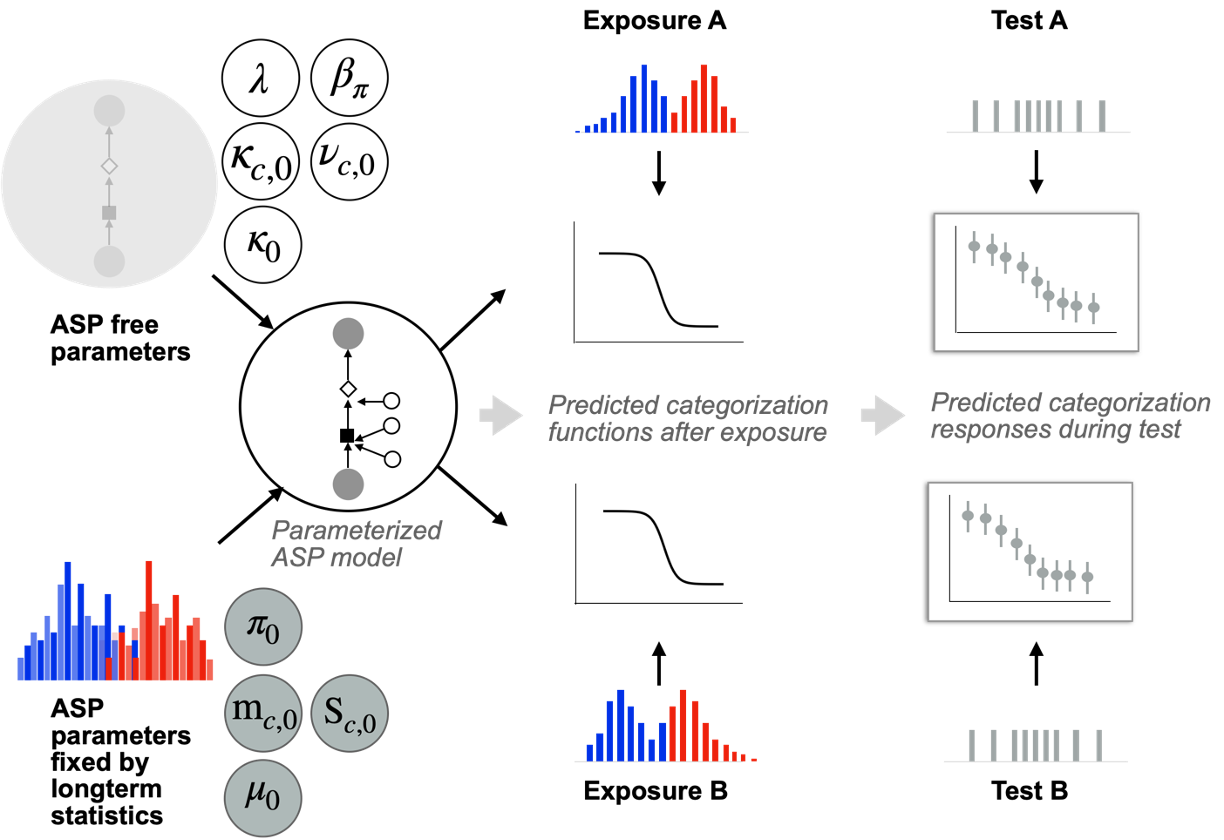
\includegraphics{../figures/diagrams/predictive-power-simulations.png}
\caption{The ASP framework can be used to derive predictions, or to fit to human behavior. ASP's change models describe how ASP's categorization model is predicted to change based on the inputs experienced during exposure. The updated categorization model can then be used to predict listeners' response distributions for any test token (as we do in Case Study 1), and/or to predict listeners' recognition accuracy (as we do in Case Study 2). As described in the text, researchers can choose to set some of ASP's parameters based on phonetic databases. By doing so, researchers commit to the assumptions (i) that listeners learn and store some statistics of previously experienced speech input, and (ii) that the database is a sufficiently good approximation of those statistics for an average listener in the experiment. Setting parameters based on phonetic databases reduces the degrees of freedom and functional flexibility of ASP's change models, leading to stronger (more easily falsifiable) predictions. This is the approach we employ in our case studies.}\label{fig:ASP-predictions}
\end{center}
\end{figure}

ASP can be used to predict changes in perception from \emph{weighted combinations} of all three change mechanisms. In the general discussion, we outline why this ability to make predictions based on combinations of mechanisms will likely be critical in moving the field forward. In that context, we discuss how future work can use ASP to address more advanced questions about the factors that determine the relative engagement of the three mechanisms---by investigating how the ASP parameters (\(\kappa_0\), \(\kappa_{c,0}\), \(\nu_{c,0}\), and \(\beta_{\pi}\)) that best explain human behavior depend on factors such as stimulus properties, task demands, and individual differences between listeners.

For our two case studies, however, we deliberately consider ASP models that employ one of the three change mechanisms at a time. This allows us to assess which of the three mechanisms are \emph{sufficient} and which ones are \emph{insufficient}, to explain the signature results of the two paradigms. Of particular theoretical interest is whether it is indeed the case that the least parsimonious change model, changes in category representations, is the only model that can explain the signature results of both perceptual recalibration and accent adaptation paradigms (as seems to be often assumed).

Beyond this specific question, we use the two case studies to (i) illustrate how intuitions about the types of results each mechanism can(not) account for are often misleading, and (ii) show how ASP can be used to inform researchers' intuitions, by predicting the effects of recent exposure on subsequent speech perception. For these reasons, both case studies focus on \emph{qualitative comparison} of ASP's predictions against the signature results from each paradigm, documented in previously published perception experiments. In the general discussion, we show how ASP can be used to compare change models in terms of their \emph{quantitative fit} against listeners' behavior.

The two case studies build on each other, each introducing new insights. Experiments on perceptual recalibration often use comparatively simple stimulus designs, intended to elicit simple boundary shifts along a uni-dimensional perceptual continuum. And while the specific tasks employed during exposure and test can vary across studies, the general stimulus design is remarkably similar across experiments. This allows us to use Case Study 1 to introduce many of the relevant concepts while keeping the paradigm comparatively simple. Case Study 2 then introduces additional complexities that come with modeling \emph{natural} accents, which can deviate from listeners' expectations in heterogeneous ways across multiple acoustic-phonetic dimensions. This additional complexity has caused researchers to question whether the same mechanisms that underlie perceptual recalibration also underlie adaptation to natural accents \autocites[see recent reviews,][]{baeseberk2018,bent-baeseberk2021,zheng-samuel2020}. Case Study 2 sheds new light on this question by asking whether even simple changes in decision-making or normalization can suffice to explain accent adaptation. Additionally, Case Study 2 allows us to illustrate an important consideration for future work: while all three change mechanisms predict that exposure should facilitate---or at least not hinder---subsequent processing of the same accent, the exact effects of exposure are predicted to depend on the specific accent properties and how they relate to listeners' prior expectations. In the general discussion, we elaborate on this point and how future work can draw on it.

\hypertarget{sec:PR}{%
\section{Case Study 1: perceptual recalibration}\label{sec:PR}}

In a typical perceptual recalibration experiment, participants are randomly assigned to one of two exposure groups that subsequently perform the same test. During exposure, participants hear stimuli that contain a critical phonetic contrast \autocite[e.g., syllable-intial /d/ vs.~/t/, as in \emph{croco\emph{d}ile} or \emph{cafe\emph{t}eria},][]{kraljic-samuel2006}, mixed with many fillers that do not contain that phonetic contrast. Between participants, critical exposure stimuli are manipulated with the goal to shift the category boundary along the phonetic contrast into different directions. This is achieved by exposing listeners to \emph{typical} pronunciations from one category and pronunciations of the other category that are acoustically \emph{shifted} towards the point of maximal perceptual ambiguity between the two categories. Which of the two categories is shifted is manipulated between the two exposure groups. To ensure that the shifted stimuli are still recognized as instances of the intended category, exposure stimuli are typically lexically or visually \emph{labeled} (e.g., hearing the shifted sound /?dt/ embedded in the lexical context of ``croco\_ile'' would label the shifted sound as a /d/). In a subsequent test phase, both groups of participants then categorize the same test stimuli along an artificially generated acoustic continuum between the two categories. The goal of this test phase is to estimate participants' categorization function for the critical phonetic contrast, and so test stimuli are \emph{unlabeled}. This is achieved by presenting the manipulated continuum in the contexts of a lexical minimal pair (e.g., \emph{dip}-\emph{tip}) or a nonce-word pair (e.g., \emph{idi}-\emph{iti}).

For example, an influential study by \textcite{kraljic-samuel2006} exposed participants to either shifted /d/ and typical /t/ or shifted /t/ and typical /d/. Participants heard 20 typical and 20 shifted tokens (mixed with 160 fillers). Following exposure, participants in both conditions categorized non-word tokens (/\ipatext{ɪ}d\ipatext{ɪ}/-/\ipatext{ɪ}t\ipatext{ɪ}/) tokens along a six-step /d/-/t/ continuum. Figure \ref{fig:kraljic-samuel-2007-replotted} shows the results obtained by Kraljic and Samuel (2006).\footnote{We estimated the VOT range in Figure \ref{fig:kraljic-samuel-2007-replotted} based on the observation that post-burst aspiration accounts for about \(2/3^{rd}\)s of the stop durations reported in Kraljic and Samuel (2007, p.~6). We also averaged over the two talkers employed in the study, as Kraljic and Samuel did not report results relative to talker-specific VOT ranges.} Although relatively small, a significant perceptual recalibration effect was observed: participants in the /d/-shifted exposure condition were more likely to give ``d''-responses, resulting a categorization function that is shifted rightwards relative to participants in the /t/-shifted condition. This shift in the category boundary is the hallmark of perceptual recalibration experiments.



\begin{figure}

{\centering \includegraphics{../figures/knitted/kraljic-samuel-2007-replotted-1} 

}

\caption{Categorization functions observed during the test phase of the perceptual recalibration experiment presented in Kraljic and Samuel (2006; replotted from Kraljic \& Samuel, 2007, Figure 1). No error bars were provided in the original, and the original data are no longer available (Samuel, p.c.).}\label{fig:kraljic-samuel-2007-replotted}
\end{figure}

Perceptual recalibration continues to be one of the most frequently used paradigm in research on adaptive speech perception. A recent review cites over 200 studies using variants of this paradigm \autocite{theodore2021}. Boundary shifts like those in Figure \ref{fig:kraljic-samuel-2007-replotted} (though often larger) have been demonstrated for an increasing number of phonetic contrasts and languages \autocites[e.g.,][]{hanulikova-weber2012,kraljic-samuel2005,kraljic-samuel2006,reinisch2013,sumner2011,vroomen2007}. We now know that boundary shifts can occur for both isolated and connected speech \autocites[e.g.,][]{eisner-mcqueen2005,reinisch-holt2013}, even after fewer shifted tokens \autocites[e.g., as few as four,][]{liu-jaeger2018,liu-jaeger2019} or under cognitive load \autocites{baart-vroomen2010,zhang-samuel2014}[but see][]{samuel2016}, and that they can persist over hours and days \autocite{eisner-mcqueen2006,vroomen-baart2009,saltzman-myers2021} though they eventually decay \autocite{samuel2021,zheng-samuel2023}. More recent work has begun to identify the brain regions involved in perceptual recalibration, which range from primary auditory cortex and superior temporal cortices to more frontal and parietal areas \autocites{bonte2017,kilianhutten2011,myers-mesite2014,ullas2020,luthra2020a}[for review, see][]{guediche2014}.

While the signature boundary shift observed in perceptual recalibration experiments is often considered the consequence of representational changes, it is also possible that this finding is compatible with explanations in terms of either of the two alternative change mechanisms. We use ASP to assess this possibility. Specifically, we predict changes in categorization following the type of exposure employed in experiments on perceptual recalibration, while switching on and off the three different change models of ASP.

\hypertarget{data}{%
\subsection{Data}\label{data}}

Most published experiments on perceptual recalibration do \emph{not} measure and report the acoustic properties of their stimuli. We therefore simulate an example experiment on perceptual recalibration to shifted /d/ and /t/, following the same stimulus creation and selection procedure employed in experiments on perceptual recalibration \autocite[e.g.,][]{kraljic-samuel2006}.\footnote{A reviewer pointed out that perceptual recalibration to shifted /d/ or /t/ does not appear to be talker-specific (for L1-US English listeners): listeners that are exposed to one talker with shifted /d/ or /t/ generalize perceptual recalibration to test tokens from a different talker \autocite[unlike for shifted /s/ or /\ipatext{ʃ}/, e.g.,][]{kraljic-samuel2007}. We consider questions about talker-specificity to be orthogonal to the questions discussed here: any of the three mechanisms integrated in ASP can be talker-specific or talker-independent, or talker-specificity can depend on the type of phonetic contrast or the type of cue (for further discussion, see SI \ref{sec:cautionary-note}).} The details of our stimulus generation approach are described in the SI (\ref{sec:SI-PR}), and do not affect the general results presented below. They are merely meant to provide a sufficiently concrete example. Readers can revisit any of the assumptions we made by downloading the \href{https://osf.io/q7gjp/}{R markdown document that this article is generated from}.

\hypertarget{exposure-phase}{%
\subsubsection{Exposure phase}\label{exposure-phase}}

Figure \ref{fig:PR-exposure-test-plot} shows the stimuli for the exposure and test phases of the experiment. During /d/-shifted exposure, listeners hear \texttt{20} lexically-labeled word recordings containing /d/ shifted towards /t/ and \texttt{20} lexically-labeled word recordings containing typical /t/, mixed in with word and non-word fillers for a total of 200 recordings. As is typical for perceptual recalibration experiments, these fillers are assumed not to contain any information about the VOT distributions of /d/ and /t/, and thus do not affect listeners' beliefs about those distributions. During /t/-shifted exposure, participants hear lexically-labeled \texttt{20} word recordings containing /t/ shifted toward /d/ and \texttt{20} lexically-labeled word recordings containing typical /d/. Shifted recordings are selected to be perceptually half-way between /d/ and /t/.



\begin{figure}

{\centering \includegraphics{../figures/knitted/PR-exposure-test-plot-1} 

}

\caption{Distribution of the exposure and test of the perceptual recalibration experiment. \textbf{Panel A - Exposure:} 20 tokens each of shifted and typical /d/ and /t/, respectively. Arrows indicate how the shifted tokens created by the experimenter differ from typical tokens of the same category (arrows originate from the mean of typical tokens and end at the mean of shifted tokens). As would be expected given the procedures researchers typically employ to generate stimuli for this type of experiment, the exposure distributions for /d/ and /t/ in both conditions differ primarily along VOT but, notably, \emph{also} differ along f0. \textbf{Panel B - Test (identical for both exposure groups):} Numbers indicate the item ID of the test tokens used in subsequent plots, with IDs in increasing order corresponding to 85\%, 65\%, 55\%, 45\%, 35\%, 15\% expected /d/-responses \emph{prior to exposure} (e.g., in a test-only norming experiment).}\label{fig:PR-exposure-test-plot}
\end{figure}

\hypertarget{test-phase}{%
\subsubsection{Test phase}\label{test-phase}}

The test phase consists of the six stimuli shown in Figure \ref{fig:PR-exposure-test-plot}B, chosen to yield 15\%, 35\%, 45\%, 55\%, 65\%, 85\% expected /d/-responses in a norming experiment without any prior exposure to the talker's speech. This closely resembles the test stimulus placement typical for perceptual recalibration experiments, which tend to examine tokens at the two ends of the continuum as well as those placed near the category boundary.

\hypertarget{results}{%
\subsection{Results}\label{results}}

Next, we use ASP to illustrate the extent to which changes in representations, response biases, or normalization can explain the typical behavioral signature of perceptual recalibration experiments: a shift in the category boundary in the same direction as the shifted tokens during exposure (optionally accompanied by a change in the slope of the categorization functions). The goal of these computational demonstrations is to illustrate the general type of pattern that the three different hypotheses can account for. Since the results of our computational demonstrations refer to the different change models introduced in Section \ref{sec:framework}, we summarize the complete ASP model in Figure \ref{fig:graphical-model-all}.

\begin{figure}
\centering
   \tikz{ %
    \node[obs] (r) {$r$} ; %
    \node[det, below=of r] (decision) {} ; %
    \factor[below=of decision, xshift=-.009cm, yshift=-.5cm] {response-dist} {left: $\mathcal{M}$} {} {}; %
% Change model for response biases
    \factor[right=of response-dist, xshift=.8cm, yshift=-2cm] {prior-dist} {left: Multi} {} {}; %
    \factor[below=of response-dist, xshift=-.009cm, yshift=-3cm] {multi} {left: Multi} {} {}; %
    \node[latent, right=of response-dist, xshift=1.95cm] (l) {$\lambda$} ; %
    \node[const, right=of l, xshift=-.009cm] (lapse) {{\em lapse rate} ($1$ DF)} ; %
    \node[det, right=of prior-dist, xshift=.4cm, yshift=-.009cm] (pi_n) {$\pi_{c,N}$} ; %
    \node[latent, right=of pi_n, yshift=1cm] (beta) {$\beta_{\pi}$} ; %
    \node[right=of beta] (beta_description) {{\em learning rate for changes in response biases} ($1$ DF)} ;
    \node[det, below=of beta, yshift=.5cm] (surprisal_i) {$I_{c_{N} | x_{N}}$} ; %    
    \node[obs, right=of surprisal_i, yshift=.5cm] (x_i) {$x_{N}$} ; %
    \node[right=of x_i, xshift=-.5cm] (x_i_description) {{\em acoustic inputs from unfamiliar talker}} ;
    \node[obs, right=of surprisal_i, yshift=-.5cm] (c_i) {$c_{N}$} ; %
    \node[right=of c_i, xshift=-.5cm] (c_i_description) {{\em category labels of acoustic inputs}} ;
  % edges
    \edge {decision} {r} ; 
    \edge {response-dist} {decision} ; %
    \edge {multi} {response-dist} ; %
    \edge {prior-dist} {response-dist} ; %
    \edge {prior-dist} {multi} ; %
    \edge {l} {response-dist} ; %
    \edge {pi_n} {prior-dist} ; 
    \edge {beta} {pi_n} ; %
    \edge {surprisal_i} {pi_n} ;
    \edge {x_i} {surprisal_i} ; %
    \edge {c_i} {surprisal_i} ; %

%change model of representations 
    \factor[below=of multi,  yshift=-4.5cm] {x_prime} {left:$\mathcal{N}$} {} {}; %
     %\node[above=of x_prime] (dots) {$\vdots$} ; %
    \node[det, right=of x_prime, yshift=2cm] (mu_n) {$\mu_{c,N}$} ; %
    \node[det, right=of x_prime, yshift=-2cm] (sigma_n) {$\Sigma_{c,N}$} ; %
% Change model for mean
    \node[latent, right=of mu_n, yshift=.75cm] (m_0) {${\rm m}_{c,0}$} ; %
    \node[right=of m_0] (m_0_description) {{\em prior beliefs about category mean} ($jk$ DF)} ;
    \node[latent, above=of m_0, yshift=-.5cm] (kappa_0) {$\kappa_{c,0}$} ; %
    \node[right=of kappa_0] (kappa_0_description) {{\em strength of prior beliefs about category mean} (up to $j$ DF)} ;
    \node[obs, right=of mu_n, yshift=-.75cm] (xbar) {$\bar{x_c}$} ; %
    \node[right=of xbar, xshift=.009cm] (xbar_description) {{\em category mean observed from unfamiliar talker}} ;
    \node[obs, below=of xbar, yshift=.5cm] (n) {$N_c$} ; %
    \node[right=of n] (n_description) {{\em number of observations for category from unfamiliar talker}} ;
% Change model for covariance
    \node[latent, right=of sigma_n, yshift=-.75cm] (s_0) {${\rm S}_{c,0}$} ; %
    \node[right=of s_0] (sigma_0_description) {{\em prior beliefs about category covariance matrix} (up to $\frac{j}{2}(k^2+k)$ DF)} ;
    \node[latent, below=of s_0, yshift=.5cm] (nu_0) {$\nu_{c,0}$} ; %
    \node[right=of nu_0] (nu_0_description) {{\em strength of prior belief about category covariance} (up to $j$ DF)} ;
    \node[obs, right=of sigma_n, yshift=.75cm] (sbar) {${\rm S}_c$} ; %
    \node[right=of sbar] (sbar_description) {{\em category sums of squares observed from unfamiliar talker}} ;
% edges
    \edge {x_prime} {multi} ; %
    \edge {mu_n} {x_prime} ; %
    \edge {sigma_n} {x_prime} ; %
    \edge {m_0} {mu_n} ; %
    \edge {kappa_0} {mu_n} ; %
    \edge {xbar} {mu_n} ; %
    \edge {sbar} {sigma_n} ; %
    \edge {s_0} {sigma_n} ; %
    \edge {nu_0} {sigma_n} ; %
    \edge {n} {mu_n} ; %
    \edge {n} {sigma_n} ; %

%Change model for normalization
    \node[det, below=of x_prime, yshift=-6cm] (x_prime2) {} ; %
    \node[obs, below=of x_prime2] (x) {x} ; %
    %\node[above=of x_prime2] (dots) {$\vdots$} ; %
    \node[det, right=of x_prime2] (mu_n) {$\mu_N$} ; %
    \node[obs, right=of mu_n, yshift=-.75cm] (xbar) {$\bar{x}$} ; %
    \node[right=of xbar, xshift=.009cm] (xbar_description) {{\em cue mean observed from unfamiliar talker}} ;
    \node[obs, below=of xbar, yshift=.75cm] (n) {$N$} ; %
    \node[right=of n] (n_description) {{\em number of observations from unfamiliar talker}} ;
    \node[latent, right=of mu_n, yshift=.75cm] (mu_0) {$\mu_0$} ; %
    \node[right=of mu_0, xshift=.1cm] (mu_0_description) {{\em prior beliefs about cue mean} ($k$ DF)} ;
    \node[latent, above=of mu_0, xshift=.009cm, yshift=-.75cm] (kappa_0) {$\kappa_0$} ; %
    \node[right=of kappa_0] (kappa_0_description) {{\em strength of prior beliefs about cue mean} ($1$ DF)} ; 
    
%edges
    \edge {x} {x_prime2} ; %
    \edge {x_prime2} {x_prime} ; %
    \edge {mu_n} {x_prime2} ; %
    \edge {mu_0} {mu_n} ; %
    \edge {kappa_0} {mu_n} ; %
    \edge {xbar} {mu_n} ; %
    \edge {n} {mu_n} ; %
}
\caption{Graphical representation of ASP, combining the categorization model from Figure \ref{fig:model-perceptual-decision-making} with the three change models from Figures \ref{fig:graphical-model-changes-normalization}, \ref{fig:graphical-model-changes-representations}, and \ref{fig:graphical-model-changes-decision-making}.}\label{fig:graphical-model-all}
\end{figure}

All three change models start from the same prior state. Specifically, we assume that listeners have acquired category representations with expected category means (\(\mathbf{E}(\mu_{/d/}), \mathbf{E}(\mu_{/t/})\)) and variances (\(\mathbf{E}(\sigma_{/d/}), \mathbf{E}(\sigma_{/t/})\)) that reflect the talker-normalized distributions in Chodroff and Wilson (2018; see Figure \ref{fig:show-representations-plots}). Prior to any exposure, decision-making is assumed to employ uniform response biases (\(\pi_{/d/}=\pi_{/t/}=.5\)). Here and throughout this article, we marginalize over the expected consequences of perceptual noise, attentional lapses, and decision-making (both for adaptation during exposure and for categorization during test). This can be seen as predicting the state of an `average' listener after exposure to a specific set of stimuli.\footnote{For any particular experiment, however, researcher have to \emph{estimate}, e.g., participants' categorization functions from their categorization responses. This is important to keep in mind, for example, when using ASP to estimate the statistical power of an experiment. To support predictive power simulations, the ASP functions provided on OSF also allow simulations that \emph{sample} the effects of perceptual noise, attentional lapses, and decision-making for adaptation and categorization. This allows simulations of trial-level behavior for individual participants.} The findings we present below do not qualitatively depend on these specific assumptions.

Finally, we note that our simulations predict categorization at the \emph{beginning} of the test phase, prior to repeated testing. This should be kept in mind when comparing our results against previous work, including the results of \textcite{kraljic-samuel2007} in Figure \ref{fig:kraljic-samuel-2007-replotted}. As is typical for experiments on perceptual recalibration, participants in Kraljic and Samuel's experiment heard the same six test tokens many times. In their visualizations and analyses, Kraljic and Samuel averaged participants' responses across these repetitions. While this approach continues to be the norm, it is now known to underestimate the true boundary shift, as repeated testing \emph{reduces} the effects of exposure \autocites{mitterer2011-perceptual-recalibration,liu-jaeger2018,liu-jaeger2019,scharenborg-janse2013,zheng-samuel2023}[for early discussion, see][p.~11]{norris2003}.

\hypertarget{changes-in-representations}{%
\subsubsection{Changes in representations}\label{changes-in-representations}}

We begin by modeling exposure-driven changes in the mapping from VOT and f0 to the /d/ and /t/ categories. This is arguably the mechanism that is most commonly assumed to underlie the boundary shift observed in perceptual recalibration experiments. Specifically, we use the \(\mathcal{NW}^{-1}\) ideal adaptor model described in Section \ref{sec:ideal-adaptor} while varying the \(\kappa_{c,0}\) and \(\nu_{c,0}\) parameters. We set the other two parameters of the \(\mathcal{NW}^{-1}\) ideal adaptor (\(\mathrm{m}\) and \(\mathrm{S}\)) so that they match the expected mean and covariance of the data in \textcite{chodroff-wilson2018} (as we did in Section \ref{sec:ideal-adaptor}). Normalization and response biases did not change based on exposure (\(\kappa_0 = \infty\); \(\beta_{\pi}=0\)), and attentional lapses were assumed to be zero (\(\lambda = 0\)).

Figure \ref{fig:PR-result-changes-in-representations} shows the predicted categorization functions after /d/-shifted and /t/-shifted exposure, depending on the strength of the prior beliefs for the category means and variances. We show the results for \(\kappa_{c,0}\)s and \(\nu_{c,0}\)s ranging from 1024 (very slow learning) to 4 (very fast learning). These values are best understood in the context of the number of critical exposure stimuli. Given 20 exposure tokens for each category, a \(\kappa_{c,0}=20\) would mean that the listeners' beliefs about the distribution of the category mean after exposure is a 50/50 mix of their beliefs prior to exposure and the mean of the exposure stimuli (see Equation \eqref{eq:niw-updating}). For \(\kappa_{c,0}=4\), listeners' beliefs about the category mean are thus primarily determined by the mean of the exposure stimuli, whereas a \(\kappa_{c,0}=1024\) essentially means that exposure does not affect listeners' belief about the category mean at all (and mutatis mutandis, for \(\nu_{c,0}\)).



\begin{figure}

{\centering \includegraphics{../figures/knitted/PR-result-changes-in-representations-1} 

}

\caption{Predictions of a learning model that derives perceptual recalibration as changes in category representations. Predicted categorization responses are shown for the 6 test tokens after /d/- and/t/-shifted exposure, depending on the strength of the prior beliefs in categories means (\(\kappa_{c,0}\)) and covariances (\(\nu_{c,0}\)). Smaller \(\kappa_{c,0}\) and \(\nu_{c,0}\) indicate \emph{faster} learning, weighting previous long-term experience less during the integration with the observations made during the exposure phase of the experiment (see Equation \eqref{eq:niw-updating}). The highlighted panel corresponds to the best-fitting \(\kappa_{c,0}\) and \(\nu_{c,0}\) observed in previous work within other types of paradigms \autocite{kleinschmidt-jaeger2016cogsci,kleinschmidt2020}.}\label{fig:PR-result-changes-in-representations}
\end{figure}

Figure \ref{fig:PR-result-changes-in-representations} demonstrates that distributional learning can account for the typical result of perceptual recalibration experiments. Of note, the range of parameterizations that best fit human responses in a series of distributional learning experiments on /b/ and /p/ \autocite[gray panel in Figure \ref{fig:PR-result-changes-in-representations}, \(\kappa_{/b/,0}=\kappa_{/p/,0}=160\) (95\% CI: 75-780) and \(\nu_{/b/,0}=\nu_{/p/,0}=510\) (95\% CI: 160-1000),][]{kleinschmidt2020} also provides a good qualitative fit against the /d/-/t/ perceptual recalibration results by Kraljic and Samuel \autocite*{kraljic-samuel2007}.

Figure \ref{fig:PR-result-changes-in-representations} further shows that boundary shifts can result from either changes in the beliefs about category means (small \(\kappa_{c,0}s\), e.g.~right column of Figure \ref{fig:PR-result-changes-in-representations}) or changes in the beliefs about category covariances (small \(\nu_{c,0}s\), e.g., bottom row in Figure \ref{fig:PR-result-changes-in-representations}). This replicates an observation made by Kleinschmidt and Jaeger \autocites*[p.~168]{kleinschmidt-jaeger2015}[see also][]{hitczenko-feldman2016,theodore-monto2019}, and highlights that ``category expansion'' and ``category shifts'' can both be seen as consequences of distributional learning \autocites[see also][]{bent-baeseberk2021,schertz-clare2020,hitczenko-feldman2016}. Figure \ref{fig:PR-result-changes-in-representations-categories} serves to further clarify how the different parameter settings for \(\kappa_{c,0}\) and \(\nu_{c,0}s\) affect the expected category likelihoods for a subset of the panels of Figure \ref{fig:PR-result-changes-in-representations}, leading to category shifts, expansion, shrinkage, or rotation, depending on both the model parameters and the input during exposure.



\begin{figure}

{\centering \includegraphics{../figures/knitted/PR-result-changes-in-representations-categories-1} 

}

\caption{Expected category likelihoods (based on expected category mean and covariance matrices) after exposure, depending on the exposure condition and the strength of the prior beliefs in categories means (\(\kappa_{c,0}\)) and covariances (\(\nu_{c,0}\)). Only a illustrative subset of the \(\kappa_{c,0}\) and \(\nu_{c,0}\) values from Figure \ref{fig:PR-result-changes-in-representations} are shown. Specifically, we compare scenarios with very slow changes in representations (first column), fast changes in beliefs about the category means (leading `category shifts', second and last column), and fast changes in beliefs about the category covariances (leading to `category expansions', `category shrinkage', and/or `category rotation', third and last column).}\label{fig:PR-result-changes-in-representations-categories}
\end{figure}

Finally, Figure \ref{fig:PR-result-changes-in-representations} shows that distributional learning not only predicts shifts in the category boundary but can also predict changes in the slope of those boundaries. This is evident, for example, in the top-right panel. Although such changes in slopes are often not discussed, they are present in many perceptual recalibration experiments \autocites[e.g.,][]{drouin2016,liu-jaeger2018,liu-jaeger2019,myers-mesite2014}.

\hypertarget{changes-in-decision-making}{%
\subsubsection{Changes in decision-making}\label{changes-in-decision-making}}

Next, we model the effects of changes in decision-making. Such changes have rarely been considered as an explanation for boundary shifts \autocite[but see][]{clarkedavidson2008}. In addition to varying the rate at which response biases change \(\beta_{\pi}\), we also vary the lapse rate parameter \(\lambda\). Normalization and representations did not change based on exposure (\(\kappa_0 = \kappa_{c,0} = \nu_{c,0} = \infty\)). Since the change model for decision-making is sensitive to the order of exposure stimuli (see Section \ref{sec:change-bias}), each panel of Figure \ref{fig:PR-result-changes-in-decision-making} averages over 50 simulations, each randomizing the order of exposure. We confirmed that this number of simulations was sufficient to achieve reproducible estimates for the range of \(\beta_{\pi}\)s considered here (the order-sensitivity of the change model increases for faster change rates, i.e., larger \(\beta_{\pi}\)).



\begin{figure}

{\centering \includegraphics{../figures/knitted/PR-result-changes-in-decision-making-1} 

}

\caption{Predictions of a model that derives perceptual recalibration as changes in decision-making. Predicted categorization responses are shown for the 6 test locations after /d/- and/t/-shifted exposure, depending on the rate at which response biases change (\(\beta_{\pi}\)) and the rate of attentional lapses (\(\lambda\)). The response biases towards /d/ that results from \(\beta_{\pi}\) are shown in the bottom row for each of the two exposure conditions, and are identical within each column (when all trials are lapses, as in the bottom row, the response distribution is identical to the response biases).}\label{fig:PR-result-changes-in-decision-making}
\end{figure}

Figure \ref{fig:PR-result-changes-in-decision-making} shows the effects of changes in decision-making for lapse rates ranging from negligible lapse rates (\(\lambda = .0005\), top row) to a scenario in which listeners always lapse (\(\lambda = 1\)). In the latter---rather implausible---edge case, listeners' responses only reflect response biases and are completely stimulus-independent (bottom row). For reference, lapse rates for perception experiments like the ones modeled here typically fall between 1-10\% \autocites[e.g.,][ constrained lapse rates to be \(<5\)\%]{clayards2008}[ report a best-fitting value of 5\%]{kleinschmidt-jaeger2016cogsci}.

The primary insight from Figure \ref{fig:PR-result-changes-in-decision-making} is that changes in response biases can account for the type of boundary shift that is observed in perceptual recalibration experiments. This shows that the signature result of perceptual recalibration experiments is ambiguous between two explanations that evoke very different cognitive architectures. For this case study, perhaps the closest match to the findings from Kraljic and Samuel (2006) is observed for plausible lapse rates up to 5\% and small changes in response bias (second or third column, top rows).

Figure \ref{fig:PR-result-changes-in-decision-making} also shows that changes in response biases do not necessarily result in effects that are symmetric around the uniform response biases assumed to hold prior to the experiment (\(\pi_{/d/}=\pi_{/t/}=.5\)). For example for \(\beta_{\pi} = .8\), the /d/-shifted condition results in a /d/-bias of \(\pi_{/d/}=.97\), whereas /t/-shifted condition results in \(\pi_{/d/}=.16\) (\(\neq 1 - .97\)). This type of asymmetry is a consequence of the assumption that listeners change their response biases only to the extent that their categorization is in conflict with the category label indicated in the input (e.g., when the listener hears a /t/ but the lexical context is \emph{lemona\_e}). This means that the degree to which listeners change their response biases depends on the degree to which the acoustic properties of the exposure stimuli are in conflict with the lexical contexts in which they appear.

Furthermore, Figure \ref{fig:PR-result-changes-in-decision-making} illustrates the effects of lapse rates (\(\lambda\)). The higher the lapse rate, the more strongly response biases, rather than stimulus-dependent aspects, determine the overall response pattern. This also means that it is important to keep lapse rates in mind when analyzing behavioral data. Consider, for example, a scenario in which listeners' lapse rates differ after /d/-shifted and /t/-shifted exposure---e.g., because one exposure condition resulted in a more difficult or less engaging task, or in less plausible stimuli. Compare, say, the blue line for \(\beta_{\pi} = .05\), \(\lambda = .005\) against the red line for \(\beta_{\pi} = .05\), \(\lambda = .5\). Analyses that fail to take into account the difference in lapse rates would wrongly conclude that the category representations have changed since the slopes of the categorization functions resulting from the two exposure conditions seem to differ.

\hypertarget{changes-in-normalization}{%
\subsubsection{Changes in normalization}\label{changes-in-normalization}}

Finally, we compare a model that normalizes test tokens based on the phonetic inputs experienced during exposure against a model that continues to apply normalization based on previous long-term experience. Essentially, the model that changes normalization based on the exposure tokens subtracts the cue means experienced during exposure---which varies based on the exposure condition---from that of each of the test tokens. We implement this by adjusting the cue values of the test tokens by the difference between the prior mean of cues based on previously experienced input (estimated in the SI, \ref{sec:SI-chodroff}) and the mean of cues experienced during exposure. All other parameters have the same setting as in the previous sections, except that no changes in representations or response biases are considered.

To illustrate the consequences of normalization, we vary the only parameter of our change model for normalization, the strength of prior beliefs about the cue mean, \(\kappa_0\). Figure \ref{fig:PR-test-normalization} illustrates the effect of normalization on the cue values of the test tokens. Figure \ref{fig:PR-result-changes-in-normalization} shows how the strength of prior beliefs is predicted to affect perceptual recalibration. These results show that changes in normalization can account for the signature boundary shift of perceptual recalibration experiments, paralleling the results for changes in representations and response biases.



\begin{figure}

{\centering \includegraphics{../figures/knitted/PR-test-normalization-1} 

}

\caption{Effects of changes in normalization on the perception of test locations, depending on the relative weighting of previous experience (\(\kappa_0\)) during the inference of the cue mean during exposure. Normalization based on exposure results in a shift in the perception of the test stimuli. The magnitude of that shift depends on \(\kappa_0\), with larger shifts (more learning) for smaller \(\kappa_0\) (see Equation \eqref{eq:normalization-change}). Color indicates the posterior probability of /d/ for each test token predicted by the categorization model after normalization (from red = 0 to blue = 1).}\label{fig:PR-test-normalization}
\end{figure}



\begin{figure}

{\centering \includegraphics{../figures/knitted/PR-result-changes-in-normalization-1} 

}

\caption{Predictions of a model that derives perceptual recalibration from changes in normalization. Predicted categorization responses are shown for the 6 test locations after /d/- and/t/-shifted exposure, depending on the relative weighting of previous experience (\(\kappa_0\)) during the inference of the cue mean during exposure. Smaller \(\kappa_0\) indicate faster learning.}\label{fig:PR-result-changes-in-normalization}
\end{figure}

\hypertarget{summary}{%
\subsection{Summary}\label{summary}}

We applied the three change models developed in Section \ref{sec:framework} to a (simulated) perceptual recalibration experiment. We found that all three change models can qualitatively predict the type of boundary shift characteristic of such experiments. To us, and we imagine to many other researchers, this finding is surprising. On the one hand, all three change models were designed to explain adaptive speech perception. As such, it is not surprising that all three models predict changes in the `right' direction, compared to the absence of an adaptive response---i.e., that all models change the categorization function in ways that are meant to accommodate the acoustic properties of the exposure stimuli. On the other hand, the three change mechanisms assume very different cognitive architectures, and each of the three change models is subject to different computational limitations. Specifically, the two simpler change models for normalization and decision-making involve fewer degrees of freedom, and have access to less information, compared to the change model for category representations. Recall, for example, that normalization affects cue values regardless of category membership, or that changes in decision-making can only predict additive changes in the log-odds of categorization responses (when listeners have lapse rates of 0 or 1).

Given these differences between the models, it seemed plausible that the simpler models would have insufficient functional flexibility to account for the types of boundary shifts associated with perceptual recalibration. Case Study 1 suggests that this is not the case. At least at the level of analysis that is typically applied in these experiments, the signature result of perceptual recalibration experiments therefore does \emph{not} constitute decisive evidence for changes in representations. Rather, boundary shifts could result from any of the three types of change mechanisms. This does not, of course, mean that perceptual recalibration experiments are \emph{necessarily} uninformative about the mechanisms underlying adaptive speech perception. To anticipate the general discussion, if adequate approaches to data analysis are chosen, it is possible to distinguish between the three different change mechanisms (and even combinations of them). Before we discuss what would be required to achieve this goal, we present the second case study using another common experimental paradigm.

\hypertarget{sec:AA}{%
\section{Case Study 2: accent adaptation}\label{sec:AA}}

The second paradigm we consider focuses on \emph{naturally} accented speech---e.g., dialectal \autocite{smith2014}, varietal \autocite{shaw2018}, or second language (L2) accents \autocite{bradlow-bent2008,eisner2013,sidaras2009,weil2001a}. Typically, exposure to an unfamiliar accent is compared to a control condition in which listeners are exposed to a familiar accent, most often the `standard' variety of listeners' first language (L1). Following exposure, listeners in either group are tested on the unfamiliar accent. In an influential study, \textcite{bradlow-bent2008} had listeners transcribe a total of 160 sentences of either Mandarin-accented US English or L1-accented US English, distributed over two sessions on two separate days. In a subsequent test phase, both groups transcribed Mandarin-accented sentences. Participants who were first exposed to Mandarin-accented US English were significantly more accurate during test (over 90\% accuracy compared to about 80\%). This finding has since been replicated and extended \autocite[for review, see][]{baeseberk2020}. We now know that substantially shorter exposure can lead to similarly large improvements in accuracy \autocite[e.g., 80 sentences in a single session, about 2-5 minutes of speech,][]{xie2021jep}, that these can persist over hours and days \autocite{witteman2015,xie2018lcn}, and that accent adaptation can sometimes generalize across talkers of the same or similar accents \autocites[e.g.,][]{baeseberk2013,tzeng2016,xie2021jep}.

As in the case of perceptual recalibration, accent adaptation is often attributed to changes in category representations \autocites[e.g.,][]{bent-baeseberk2021,sidaras2009,eisner2013,sumner2009,tzeng2016,xie2016jep}. This might in part be due to the intuition that the other change mechanisms are not sufficiently flexible to explain adaptation to complex differences between accents. For example, a common assumption seems to be that changes in decision/response biases can only explain \emph{trade-offs} in accuracy: as the accuracy for one category improves, it has to inevitably decrease for all other categories. Under this trade-off assumption (which we show below to be false), changes in decision-making could not possibly explain \emph{overall} improvements in recognition accuracy. Similarly, pre-linguistic normalization is rarely considered a plausible mechanism for accent adaptation. However, previous work has never actually put these intuitions to a test. Case Study 2 provides this test.

Compared to perceptual recalibration paradigms, experiments on accent adaptation exhibit more heterogeneity in their designs and tasks. Case Study 2 focuses on experiments in which treatment exposure employs a single talker with an unfamiliar accent, and the test phase heard by both groups of participants employs previously unheard stimuli from the same accented talker \autocites[e.g.,][]{eisner2013,schertz2015,xie2017}.\footnote{The approach we take here can also be applied to cross-talker generalization---i.e., paradigms in which speech from different talkers of the same (or different) accent as the exposure talker is used during test \autocite{baeseberk2013,bradlow-bent2008,sidaras2009}.} For example, in an exposure-test experiment, \textcite{xie2016jep} exposed two groups of L1-US English listeners to Mandarin-accented US English speech. In exposure, participants in the treatment group heard 30 words ending in /d/ (e.g., \emph{overload}) together with 60 word fillers and 90 nonword fillers. Participants in the control group did not hear any words that contain /d/. After exposure, participants in both conditions categorized recordings of 60 minimal /d/-/t/ pairs (e.g., \emph{seed} vs.~\emph{seat}) spoken by the same Mandarin-accented talker. Participants who heard /d/-final words during exposure were more likely to categorize /d/-final words correctly during test, compared to the control condition. At the same time, a non-significant numerical \emph{de}crease in accuracy was observed for /t/-final words \autocite[see also][]{xie2018lcn}. Related paradigms have yielded similar results for other contrasts and other L1-L2 pairs \autocites[e.g.,][]{zheng-samuel2020,eisner2013}.

For Case Study 2, we construct a hypothetical experiment that closely follows this type of design. For the sake of continuity, we focus on the same syllable-initial /d/-/t/ contrast used in Case Study 1. Specifically, we qualitatively simulate exposure to Korean-accented L2 English, which tends to weight the two cues to /d/-/t/ considered here (VOT and f0) differently than L1-US English. Like in Case Study 1, we analyze the data following the conventions of the field. For Case Study 2, this means that we assess how exposure affects L1 listeners' subsequent categorization accuracy for L2-accented test tokens. As in Case Study 1, we ask whether any of the three change mechanisms can qualitatively explain the signature results found in \textcite{xie2016jep} and other similar work. As in any experiment on accent adaptation, the results of our simulated experiment are expected to depend on the acoustic-phonetic characteristics of both the L1 and the L2 accents. In the discussion of Case Study 2, we thus consider other common differences between L1 and L2 accents, and show how these accent properties are expected to affect the three different change models.

\hypertarget{data-1}{%
\subsection{Data}\label{data-1}}

The stimulus generation procedure is described in detail in the SI (\ref{sec:SI-AA}).

\hypertarget{exposure-phase-1}{%
\subsubsection{Exposure phase}\label{exposure-phase-1}}

Figure \ref{fig:AA-exposure-test-plot}A shows the stimuli for the exposure and test phases of the experiment. In the L2-accented exposure condition, listeners hear word recordings containing L2-accented initial /d/ and /t/ (30 tokens per category). In the control condition with L1-accented exposure, listeners hear the same words but from an L1-accented talker.\footnote{The use of L1-accented exposure, rather than L2-accented exposure without /d/, as control follows a typical design in accent adaptation studies \autocite[e.g.,][]{bradlow-bent2008}, rather than \textcite{xie2016jep}. Xie and colleagues instead employed L2-accented exposure without /d/, using the same L2-accented talker as during test \autocite[see also][]{eisner2013}. For the present purpose, both types of control conditions lead to identical predictions (as long as the L2-accented control exposure successfully avoids conveying non-negligible amount of information about the categories considered during the test phase) since the current implementation of the three change models do not consider talker-switch costs.} For L1-accented exposure, the category likelihoods were set to match those observed in \textcite{chodroff-wilson2018}, after C-CuRE normalization (i.e., the distributions shown in Figure \ref{fig:demonstrate-normalization}B). This follows the same approach we took for the typical tokens in Case Study 1. For L2-accented exposure, /d/ and /t/ categories were created following the VOT and f0 statistics of Korean-accented US English reported in \textcite{schertz2015}. The /d/ and /t/ categories in this L2 accent differ from L1-accented US English in both category means and variances. First, the VOTs of both stop categories are longer in the L2 accent, making the /d/s more similar to /t/s for native-English listeners who rely on VOT as a primary cue to voicing distinction. As a result, the recognition accuracy is expected to be lower for /d/ than for /t/ for the L1-accented exposure condition. Second, the L2-accented categories exhibit the same ordering along f0 as in L1-accented US English (lower f0 for /d/ than for /t/), but this difference along f0 is enhanced in Korean-accented US English. This makes syllable-initial stop voicing in Korean-accented US English a representative case of cue reweighting, a common difference between L2 and L1 accents that has received much attention in research on accent adaptation \autocites[e.g.,][]{escudero2009,kim2020,schertz2016}[see also][]{idemaru-holt2011,idemaru-holt2020,harmon2019}.

\hypertarget{test-phase-1}{%
\subsubsection{Test phase}\label{test-phase-1}}

During test, listeners from both exposure conditions hear the same recordings from the same L2-accented talker used in the L2-accented exposure condition. 60 test tokens are randomly sampled from the distribution of each L2-accented category, half from the /d/ category and half from the /t/ category (Figure \ref{fig:AA-exposure-test-plot}B).



\begin{figure}

{\centering \includegraphics{../figures/knitted/AA-exposure-test-plot-1} 

}

\caption{\textbf{Panel A - Exposure:} Distribution of the stimuli used during the exposure phase of the accent adaptation experiment (30 tokens each of L1-accented and L2-accented /d/ and /t/, respectively). \textbf{Panel B - Test:} Distribution of the stimuli used during the test phase of the accent adaptation experiment. The test tokens come from L2-accented speech (60 tokens per category) and are identical for the two exposure conditions. Ellipses show the 95\% probability mass for the two categories in L2-accented exposure speech.}\label{fig:AA-exposure-test-plot}
\end{figure}

\hypertarget{results-1}{%
\subsection{Results}\label{results-1}}

\begin{table}

\caption{\label{tab:AA-table-models-parameter-setting}Parameter range considered for each change model}
\centering
\begin{tabular}[t]{lll}
\toprule
Model & Parameters & Range\\
\midrule
Changes in decision-making & $\lambda$ & 0 to 1\\
\cmidrule{1-3}
 & $\beta_\pi$ & 0.001 to 100\\
\cmidrule{1-3}
Changes in representations & $\kappa_{c,0}$ & 1 to 10000\\
\cmidrule{1-3}
 & $\nu_{c,0}$ & 4 to 10000\\
\cmidrule{1-3}
Changes in normalization & $\kappa_0$ & 1 to 10000\\
\bottomrule
\end{tabular}
\end{table}

Paralleling Case Study 1, we predict L1 listeners' response behavior under each of the three change models. For each change model, we evaluate whether it can explain the two types of signature results observed in, for example, Xie et al. \autocite*{xie2016jep}: (1) with L1-accented exposure, /d/ test tokens are recognized with lower accuracy than /t/ test tokens, since the categories are shifted towards /t/ along the primary cue VOT, creating a deviation from L1 listeners' expectations; and (2) L2-accented exposure should lead to a significant increase in recognition accuracy for /d/ test tokens without a corresponding decrease in the accuracy for /t/ test tokens, resulting in an overall increase in accuracy.

As in Case Study 1, we first model changes in representations, and then compare them against changes in decision-making and normalization. We consider a wider range of parameterizations than in Case Study 1, because the models with the highest accuracy for L2-accented exposure (henceforth, the best-performing parameterization) in some cases fell outside the parameter ranges considered in Case Study 1. These best-performing parameterizations were determined by bounded quasi-Newton optimization of the recognition accuracy during test after L2-accented exposure \autocite[implemented in function \texttt{optim()} in R]{byrd1995}, and are indicated in all result plots we present below. Table \ref{tab:AA-table-models-parameter-setting} summarizes the parameter ranges considered by the optimization algorithm \autocite[\(\nu_{c,0}\) must be larger than the number of cues \(k\) + 1,][p.~134]{murphy2012}.\footnote{\label{fn:optimization} For changes in decision-making, bounded quasi-Newton optimization and other optimization algorithms (implemented in \texttt{optim()}) struggled to reliably determine the best-performing parameterizations. We thus initially performed a grid search over a large range of the parameter space (defined by \(\beta_{\pi}\) and \(\lambda\)), and then started the optimization process from the best-performing parameterization in that grid.} We emphasize that we use the term ``best-performing'' to refer to the parameterization that achieves the highest recognition accuracy for L2-accented test tokens, rather than the best fit against human responses in a perception experiment. In the general discussion, we describe how the same approach can be used to fit change models to the results of perception experiments.

\hypertarget{changes-in-representations-1}{%
\subsubsection{Changes in representations}\label{changes-in-representations-1}}



\begin{figure}

{\centering \includegraphics{../figures/knitted/AA-result-changes-in-representations-1} 

}

\caption{Predictions of a learning model that derives accent adaptation as changes in category representations. Predicted categorization accuracies for the L2-accented test tokens after L1-accented or L2-accented exposure, as a function of the strength of the prior beliefs in category means (\(\kappa_{c,0}\)) and covariances (\(\nu_{c,0}\)). The average accuracy across /d/ and /t/ is shown above the bars for each exposure condition. Error bars show 95\% bootstrapped confidence intervals. The highlighted panel is the one closest to the best-performing parameterization (\(\kappa_{c,0} = 1\); \(\nu_{c,0}=4\); overall accuracy \(=0.93\)).}\label{fig:AA-result-changes-in-representations}
\end{figure}

Figure \ref{fig:AA-result-changes-in-representations} shows the predicted categorization accuracy after exposure to L1- or L2-accented speech, as a function of the strength of the prior beliefs for the category means and variances. First consider the top left panel, where both \(\kappa_{c,0}\) and \(\nu_{c,0}\) have very high values. This simulates a very slow learner with strong prior beliefs for both category means and variances, so that the small number of exposure tokens has minimal influence on subsequent perception of the L2-accented test tokens. Therefore, the performance seen in the L1- and L2-accented exposure conditions is more or less identical, reflecting how a listener would draw primarily on their long-term prior experience to categorize the test tokens.

As \(\kappa_{c,0}\) and \(\nu_{c,0}\) get smaller (indicating weaker prior beliefs), the effects of exposure become more noticeable, and both of the signature results of experiments on accent adaptation begin to emerge. First, for L1-accented exposure, the accuracy is always predicted to be lower for /d/ than for /t/, indicating that /d/ is often misheard as /t/. Second, L2-accented exposure is predicted to improve recognition accuracy of /d/ compared to L1-accented exposure, and this improvement occurs without corresponding decreases in the recognition accuracy of /t/. Looking across the range of \(\kappa_{c,0}\)s and \(\nu_{c,0}\)s, we make two more observations. First, for the scenario studied here, faster learning of category means improves recognition accuracy. When listeners' beliefs about category covariances are held constant (i.e., looking within each row), smaller \(\kappa_{c,0}\) values yield higher categorization accuracy. Second, faster updating of beliefs about the \emph{(co)variance} also leads to accuracy improvements, although these improvements are less pronounced. Both results follow from the way that the Korean-accented stimuli differ from the L1 accented stimuli: as shown in Figure \ref{fig:AA-exposure-test-plot}, the category means of Korean-accented /d/ and /t/ are shifted relative to the L1-accented stimuli. In comparison, differences in category (co)variances are relatively subtle between the two sets of stimuli. For the present exposure stimuli, adapting to the L2 accent thus primarily hinges on learning the new category means. Taken together, these results demonstrate how changes in representation can explain the types of results that are considered to be the signature of accent adaptation.

\hypertarget{changes-in-decision-making-1}{%
\subsubsection{Changes in decision-making}\label{changes-in-decision-making-1}}



\begin{figure}

{\centering \includegraphics{../figures/knitted/AA-result-changes-in-decision-making-1} 

}

\caption{Predictions of a model that derives accent adaptation as changes in decision-making. Predicted categorization accuracies for the L2-accented test tokens after L1-accented or L2-accented exposure, depending on the rate at which response biases change (\(\beta_{\pi}\)) and the rate of attentional lapses (\(\lambda\)). The highlighted panel is the one closest to the best-performing parameterization (\(\beta_{\pi} = 2.2\); \(\lambda=0\); overall accuracy\(=0.94\)).}\label{fig:AA-result-changes-in-decision-making}
\end{figure}

Figure \ref{fig:AA-result-changes-in-decision-making} shows the effects of changes in decision-making as a function of the rate at which response biases change \(\beta_{\pi}\) and the lapse rate \(\lambda\), averaged across all simulations for each parameterization. As in Case Study 1, the figure shows the average across a minimum of 50 repeated simulations, each time randomizing the order of exposure. This was sufficient to achieve reproducible estimates even for the largest \(\beta_{\pi}\)s considered here (SEs of the mean accuracy after L2-accented exposure across repeated simulations were smaller than \(0.002\), meaning that the 95\% CI across the simulations spanned less than 1\% in recognition accuracy).

For L1-accented exposure, we again see that /d/ test tokens are categorized substantially less accurately than /t/ test tokens, regardless of the specific value of \(\beta_{\pi}\). The second signature result---improved accuracy after L2-accented exposure for /d/---is obtained for sufficiently fast learning rates \(\beta_{\pi}\). As \(\beta_{\pi}\) increases, the overall recognition accuracy first increases and then decreases and finally plateaus (for details, see SI, \ref{sec:SI-grid-search}). The largest improvements are found for the smallest lapse rates and relatively fast learning rates (gray panel in Figure \ref{fig:AA-result-changes-in-decision-making}).

Importantly, Figure \ref{fig:AA-result-changes-in-decision-making} shows that changes in response biases do not necessarily result in the type of zero-sum trade-off that is sometimes attributed to them---accuracy increasing by some degree for one category while decreasing by the same degree for the other category. Rather, L2-accented exposure can predict improvements in the \emph{overall} recognition accuracy across both categories (e.g., top right panel). Zero-sum trade-offs are only expected under the highly implausible assumptions that responses are entirely independent of stimulus properties (bottom row of Figure \ref{fig:AA-result-changes-in-decision-making}). Indeed, for the specific L1-L2 accent combination considered here, the largest improvements observed for changes in decision-making are similar in magnitude to those observed for the representational change model, despite the fact that the former change model is computationally simpler.

\hypertarget{changes-in-normalization-1}{%
\subsubsection{Changes in normalization}\label{changes-in-normalization-1}}

Finally, we compare models that normalize test tokens based on the phonetic input experienced during exposure against models that continue to apply normalization based on prior long-term L1 experience. Figure \ref{fig:AA-result-changes-in-normalization} shows the predicted categorization accuracy following changes in normalization in the L1- and L2-accented exposure conditions. We again obtain both of the signature results of experiments on accent adaptation. For L1-accented exposure, we continue to see that /d/ test tokens are categorized substantially less accurately than /t/ test tokens. For L2-accented exposure, recognition accuracy is improved for /d/ test tokens without any decrease in the recognition accuracy for /t/. That is, like the other two change models, normalization can predict \emph{overall} improvements in recognition accuracy after L2-accented exposure. Indeed, for the specific L1-L2 accent combination considered here, the computationally simple model for changes in normalization yields improvements similar to those predicted by changes in category representations.



\begin{figure}

{\centering \includegraphics{../figures/knitted/AA-result-changes-in-normalization-1} 

}

\caption{Predictions of a model that derives accent adaptation from changes in normalization. Predicted categorization accuracies for the L2-accented test tokens after L1-accented or L2-accented exposure, depending on the relative weighting of previous experience (\(\kappa_0\)) during the inference of the cue mean during exposure. The highlighted panel is the one closest to the best-performing parameterization (\(\kappa_0 = 1\); overall accuracy \(=0.92\)).}\label{fig:AA-result-changes-in-normalization}
\end{figure}

\hypertarget{summary-1}{%
\subsection{Summary}\label{summary-1}}

Paralleling Case Study 1 on perceptual recalibration, we find that any of the three change mechanisms can qualitatively explain the signature results for accent adaptation---at least for the hypothetical L2 accent considered here. Although this L2 accent differs from L1 listeners' prior expectations in complex ways---specifically, the relative weighting of VOT and f0---even computationally simple, non-representational change mechanisms (normalization and decision-making) predict improved recognition accuracy after L2-accented exposure. For example, contrary to common assumptions, changes in decision-making can lead to \emph{overall} improvements in recognition accuracy, not just zero-sum trade-offs. This supports the conclusion of Case Study 1: at the level of analysis that is commonly applied in previous work (and thus in our case studies), experiments on accent adaptation do not necessarily rule out any of the three mechanisms.

For the hypothetical L2 accent considered in Case Study 2, the three change models do not only make similar \emph{qualitative} predictions (e.g., improved performance after L2-accented exposure), they also yield highly comparable \emph{quantitative} performance: recognition accuracies of the best-performing models in Figures \ref{fig:AA-result-changes-in-representations}-\ref{fig:AA-result-changes-in-normalization} range from .92 for normalization to .94 for changes in decision-making. Intuitively, quantitatively similar performance makes it particularly difficult to distinguish between the three change models, or combinations thereof.

Fortunately for research on adaptive speech perception, it is not always the case that the three change models can explain similar ranges of performance. A critical insight of ASP is that the predicted benefit of L2-accented exposure under each mechanism depends on the acoustic-phonetic statistics of the accent, relative to L1 listeners' prior expectations. For experiments using naturally accented stimuli, this means that the results are expected to depend on the specific acoustic-phonetic properties of the exposure and test tokens. To further illustrate this point, we simulated three additional scenarios, shown in Figure \ref{fig:AA-plot-results-additional-cases}A. The top row of Figure \ref{fig:AA-plot-results-additional-cases} replot the example of cue weighting presented above for comparison. Each of the three additional scenarios (2nd to bottom rows) is representative of commonly attested differences between L1- and L2-accents. The second row of Figure \ref{fig:AA-plot-results-additional-cases} shows an example of \emph{contrast reduction}, in which the L2 accent shows a greater category overlap than the L1 accent. Here it is simulated by shifting /d/ category towards /t/ along the VOT continuum while keeping the latter unchanged \autocite[as qualitatively attested for, e.g., vowels in Spanish-accented English,][]{wade2007}. The third row shows an example of \emph{contrast shift}, where two categories in L2-accented speech are shifted along one or more of the cue dimensions as compared to L1-accented speech. Here it is simulated by shifting both /d/ and /t/ categories towards lower VOT \autocite[qualitatively attested for, e.g., word-initial stops in French-accented English,][]{sumner2011}. The bottom row of Figure \ref{fig:AA-plot-results-additional-cases} shows a more extreme example, exhibiting almost complete \emph{contrast collapse} \autocite[similar to the loss of the /s/-/\ipatext{θ}/ contrast that can occur in Mandarin-accented English,][]{zheng-samuel2020}. Here it is simulated by making /d/ identical to /t/.



\begin{figure}

{\centering \includegraphics{../figures/knitted/AA-plot-results-additional-cases-1} 

}

\caption{Predicted adaptation for four types of L2 accents, from top to bottom: cue reweighting, contrast reduction, contrast shift and contrast collapse. Predictions were derived for one random experiment of the same number of exposure and test stimuli as in Case Study 2. Multiple simulations were performed following the same procedure described in the main scenario above. \textbf{Panel A - Distributions of L1-accented and L2-accented categories:} L1-accented categories, represented in light shades, are kept constant across the three scenarios and identical to that in the main scenario above; L2-accented categories, represented by solid ellipses, are varied across scenarios. \textbf{Panel B - Change model predictions:} Predicted categorization accuracies for the L2-accented test tokens after L1-accented and L2-accented exposure, for the best-performing parameterizations of each change model (cf.~highlighted panels in Figure \ref{fig:AA-result-changes-in-representations}-\ref{fig:AA-result-changes-in-normalization}). The average accuracy across all test tokens for each condition is shown above the bars. Error bars show 95\% bootstrapped confidence intervals.}\label{fig:AA-plot-results-additional-cases}
\end{figure}

\begin{table}

\caption{\label{tab:AA-table-best-performing-parameterization}Best-performing parameterizations across different accent scenarios. Recall that best-performing here refers to the parameterization that achieves the highest accuracy on L2-accented test tokens, rather than best quantitative fit against human data (which we do not have).}
\centering
\resizebox{\linewidth}{!}{
\begin{tabular}[t]{llll}
\toprule
L2 accent scenario & Changes in representations & Changes in decision-making & Changes in normalization\\
\midrule
Cue reweighting & $\kappa_{c,0}$ = 1, $\nu_{c,0}$ = 4 & $\lambda$ = 0, $\beta_\pi$ = 2.2 & $\kappa_0$ = 1\\
Contrast reduction & $\kappa_{c,0}$ = 19, $\nu_{c,0}$ = 10000 & $\lambda$ = 0, $\beta_\pi$ = 2.15 & $\kappa_0$ = 1\\
Contrast shift & $\kappa_{c,0}$ = 1, $\nu_{c,0}$ = 10000 & $\lambda$ = 0, $\beta_\pi$ = 0.16 & $\kappa_0$ = 1\\
Contrast collapse & $\kappa_{c,0}$ = 28, $\nu_{c,0}$ = 1652 & $\lambda$ = 0.1, $\beta_\pi$ = 2.75 & $\kappa_0$ = 5000\\
\bottomrule
\end{tabular}}
\end{table}

Figure \ref{fig:AA-plot-results-additional-cases}B shows how the four accent scenarios are predicted to affect L1 listeners' perception, both prior to informative exposure (L1-accented exposure condition) and after L2-accented exposure. Each panel shows the predictions of the best-performing parameterization for the change model, derived in the same way as for the cue-reweighting case described above (best-performing parameters are listed in Table \ref{tab:AA-table-best-performing-parameterization}). The results of these additional simulations serve to emphasize several important considerations for future research.

Foremost of all, Figure \ref{fig:AA-plot-results-additional-cases}B shows that the predictions of the three change mechanisms \emph{can} differ qualitatively, depending on the accent scenario. While all three change models achieve qualitatively similar accuracy for three of the four simulated accent scenarios (top, second and bottom row of Figure \ref{fig:AA-plot-results-additional-cases}B), this is not the case for our example of contrast shift (third row). For this simulated scenario, changes in category representations and normalization can yield qualitative improvements after exposure, whereas changes in decision-making do not. This shows that experiments on accent adaptation \emph{could} shed light on the underlying change mechanisms \emph{provided experimenters were to design and analyze their experiments in ways that explicitly link the acoustic-phonetic properties of the exposure and test items to participants' responses} (e.g., by selecting accent properties that are predicted to yield different adaptive responses under the three different change mechanisms). This is, however, hardly ever attempted in research on accent adaptation. The few existing exceptions, while insightful in their own right, have been limited to informal discussions of how the acoustic-phonetic properties of L1 and L2 accents might have qualitatively contributed to the results, rather than explicit comparisons of models \autocites[e.g.,][]{schertz2015,tan2021,xie2016jep}. In the general discussion, we make concrete recommendations as to how the field can move beyond this status quo.

Before we turn to these recommendations, we make two more observations about the results in Figure \ref{fig:AA-plot-results-additional-cases}B that might be of interest to researchers who plan to use ASP to design and interpret their experiments. First, accent scenarios can differ in the difficulties they are predicted to cause for L1 listeners prior to informative exposure. For example, without L2-accented exposure, contrast reduction (second row) and contrast collapse (bottom row) are predicted to cause difficulties similar to those predicted for cue reweighting (top row): L1 listeners unfamiliar with the accent are expected to struggle with the recognition of /d/ than the recognition of /t/. The opposite is observed for our example of contrast shift (third row). This illustrates how different L2 accent properties can lead to different perceptual consequences for L1 listeners.

Second, the four scenarios in Figure \ref{fig:AA-plot-results-additional-cases}A also differ in how much L2-accented exposure is predicted to affect perception. This includes differences across the accent scenarios in terms of the maximum accuracy any particular change model can achieve. For example, changes in category representations can improve recognition accuracy to \textgreater90\% for L2-accented exposure for both the example of cue reweighting and the example of contrast shift. For our example of contrast reduction, however, the improvements achievable by changes in category representations are more modest (\textasciitilde72\% after L2-accented exposure). There are even accent scenarios for which \emph{none} of the change models predicts any significant benefits from L2-accented exposure (see bottom row of Figure \ref{fig:AA-plot-results-additional-cases}B). This highlights an important, yet often under-appreciated, fact: sometimes null results are \emph{predicted} because of the specific stimulus statistics \autocites[see][]{tan2021,zheng-samuel2020}. Put differently, an absence of improvements does not \emph{necessarily} constitute evidence against accent adaptation or any of the three mechanisms.

The scenarios considered here only cover a subset of the L2 accent properties that exist in the world. They suffice, however, to illustrate a general challenge: different types of cross-talker differences---including L2 accents---pose different types of challenges to listeners (this is further reflected in the fact that the best-performing parameterizations for the same mechanism vary across the different accent scenarios, cf.~Table \ref{tab:AA-table-best-performing-parameterization}). It follows that, depending on the specific accent properties, listeners can benefit from different engagement of the three mechanisms \autocite[and different rates of adaptation, see discussion of the flexibility-stability trade-off in][pp.~180-182]{kleinschmidt-jaeger2015}. This means that differences between accents can be a natural testbed for distinguishing between hypotheses about the change mechanisms affording adaptive speech perception. In the general discussion, we explore how such tests can be accomplished.

\printbibliography
\erefsection

\brefsection

\printbibliography
\erefsection


\printbibliography

\end{document}
